\chapter{Resultados}

Nesse capítulo a ferramenta será demonstrada, realizando-se projetos de exemplo a fim de demonstrar seu funcionamento e permitir a realização de comparações com as ferramentas já existentes.

\section{A Ferramenta}

\begin{figure}[H]
  \centering
  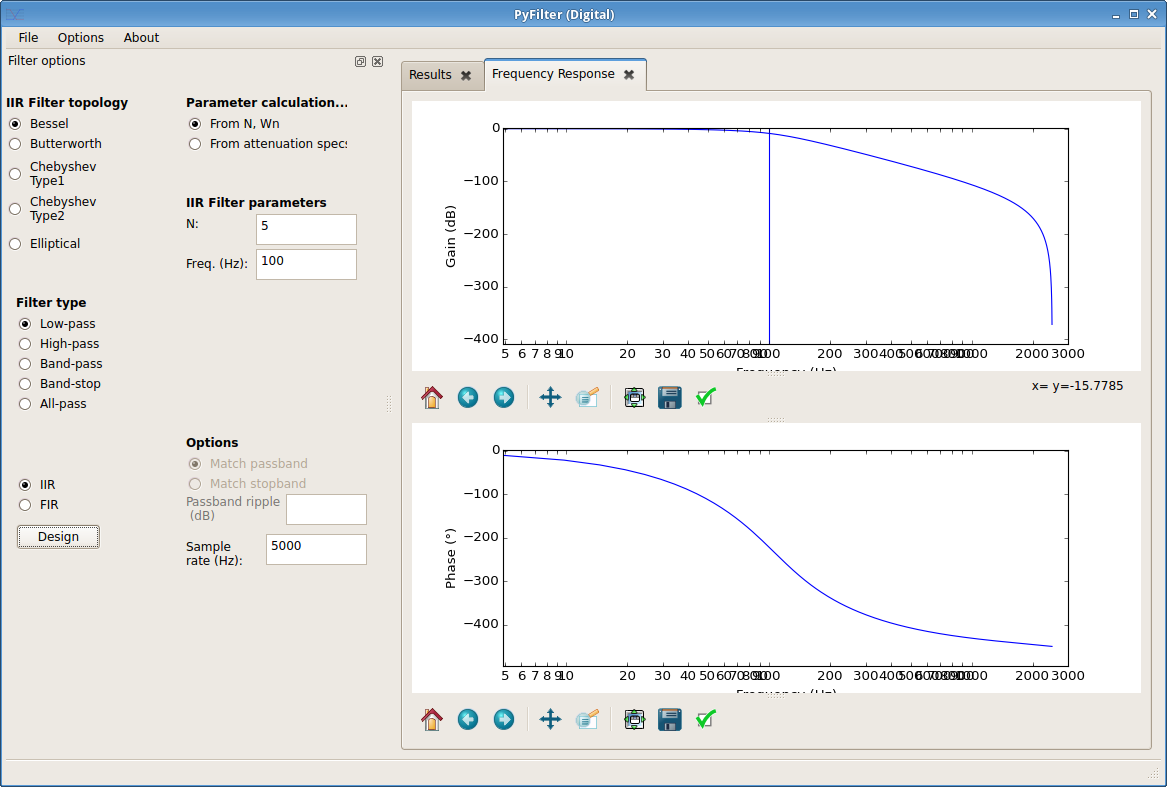
\includegraphics[scale=0.4]{images/screens/pyfilter_digital_gui}
  \caption{Interface gráfica da ferramenta, para projeto de filtros digitais. }
  \label{fig:pyfilter_gui}
\end{figure}

\begin{figure}[H]
  \centering
  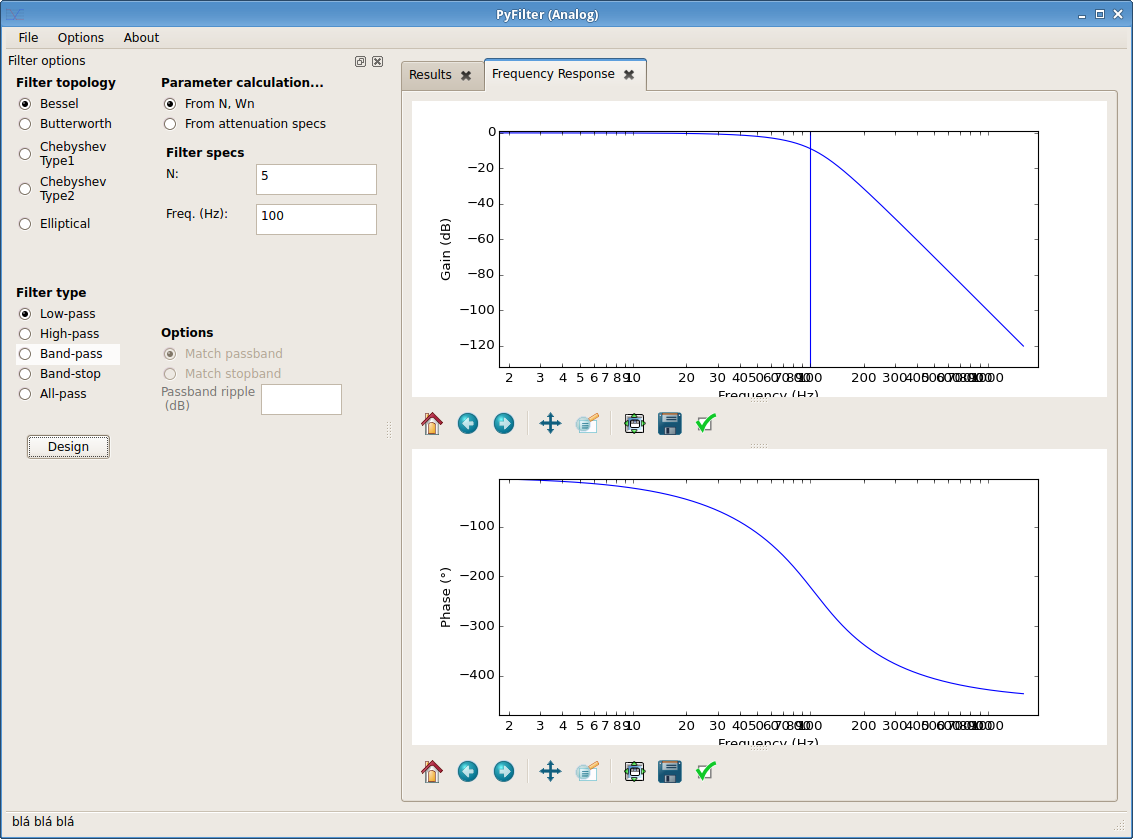
\includegraphics[scale=0.4]{images/screens/pyfilter_analog_gui}
  \caption{Interface gráfica da ferramenta, para projeto de filtros analógicos.}
  \label{fig:pyfilter_analog_gui}
\end{figure}


Nas figuras \ref{fig:pyfilter_gui} e \ref{fig:pyfilter_analog_gui}, apresenta-se a interface gráfica da ferramenta desenvolvida. Seu uso é bastante direto: o usuário irá selecionar e entrar com os parâmetros do filtro desejado, e após selecionada a opção de projetar o filtro, será apresentado um relatório com a função de transferência e os coeficientes, além das respostas de magnitude e fase para o filtro projetado.

\section{Exemplo de projeto: filtro passa-baixa}
\label{sec:lowpass}
Em \cite{sancho} temos o exemplo de projeto de um filtro passa-baixa para aplicação biomédica, na qual é desejada uma frequência de corte muito baixa (8 mHz). A realização deste projeto demonstra-se uma tarefa desafiadora devido aos valores dos componentes envolvidos; no mesmo artigo encontram-se propostas de topologias de circuitos para solução desses problemas, porém que já fogem ao objetivo do presente trabalho.

\subsection{Projeto Analógico}
No artigo original, é implementado um filtro Butterworth de segunda ordem devido à característica de planicidade desejável à aplicação deste; aqui, foram implementados filtros de quarta ordem em todas as topologias expostas na introdução. Dessa forma, obtém-se as seguintes curvas para os filtros projetados:

\begin{figure}[H]
  \centering
  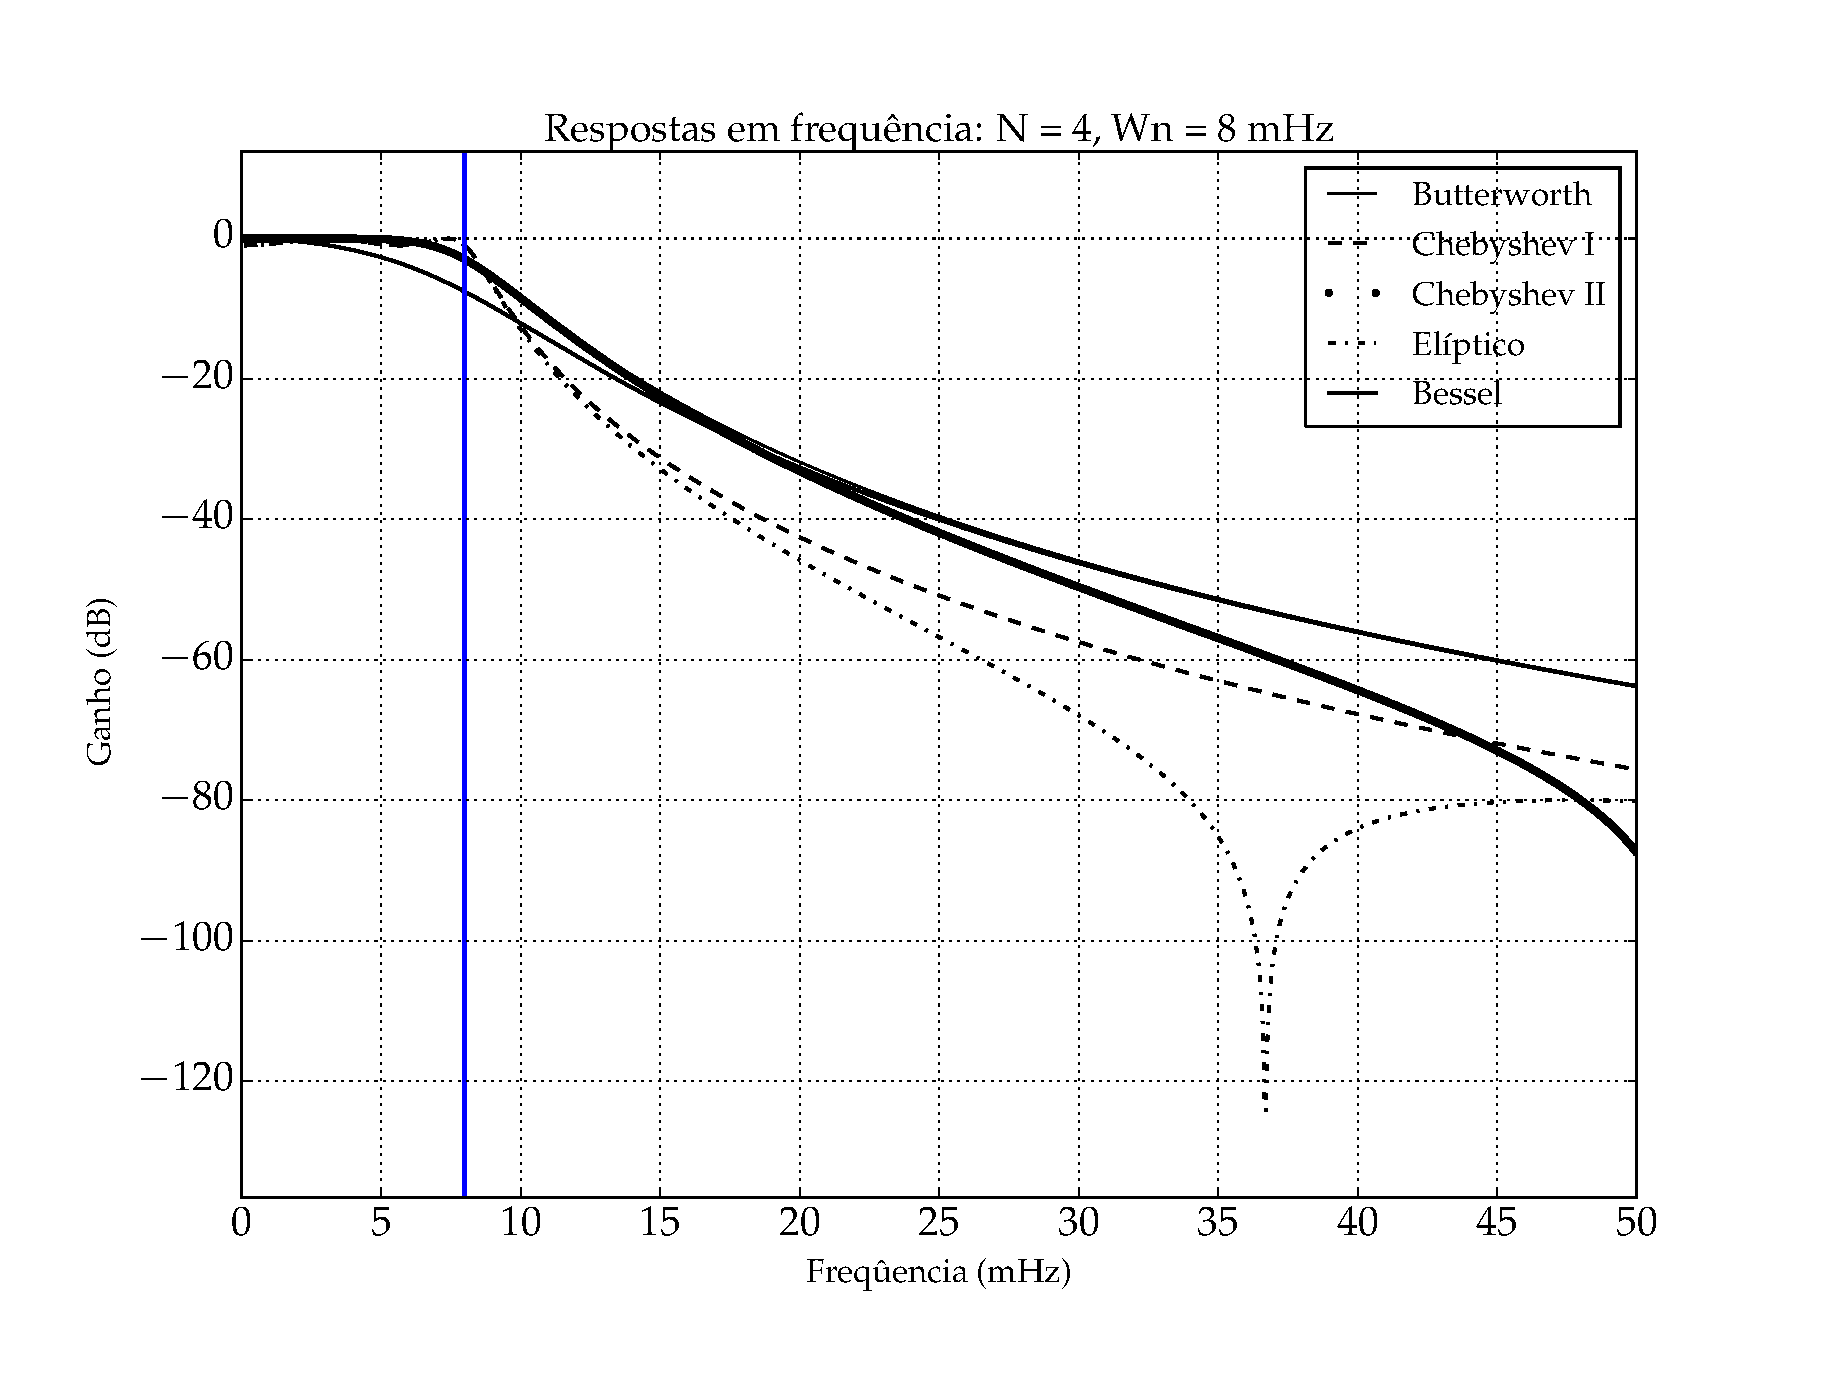
\includegraphics[scale=0.55]{images/plots/lowpass_analog}
  \caption{Resposta em frequência para filtro low-pass analógico. }
  \label{fig:lowpass_analog_response}
\end{figure}


A partir do resultado obtido, é possível verificar aquilo que foi afirmado na fundamentação teórica deste trabalho: filtros Butterworth e Bessel tem uma maior planicidade na banda de passagem, ao passo que os filtros Chebyshev apresentam uma transição mais rápida ao custo de terem maior \textit{ripple}. Constata-se também que, para uma frequência $f \gg f_c$, o filtro de Bessel aproxima o filtro de Butterworth.

\subsection{Projeto Digital: IIR}
Inicialmente, foi tentada uma taxa de amostragem de 1000 Hz, todavia constatou-se que esta era inadequada para a aplicação, pois os coeficientes dos filtros efetivamente tornavam-se zero. Então, estabeleceu-se para este projeto que a taxa de amostragem será de 5 Hz.

\begin{figure}[H]
  \centering
  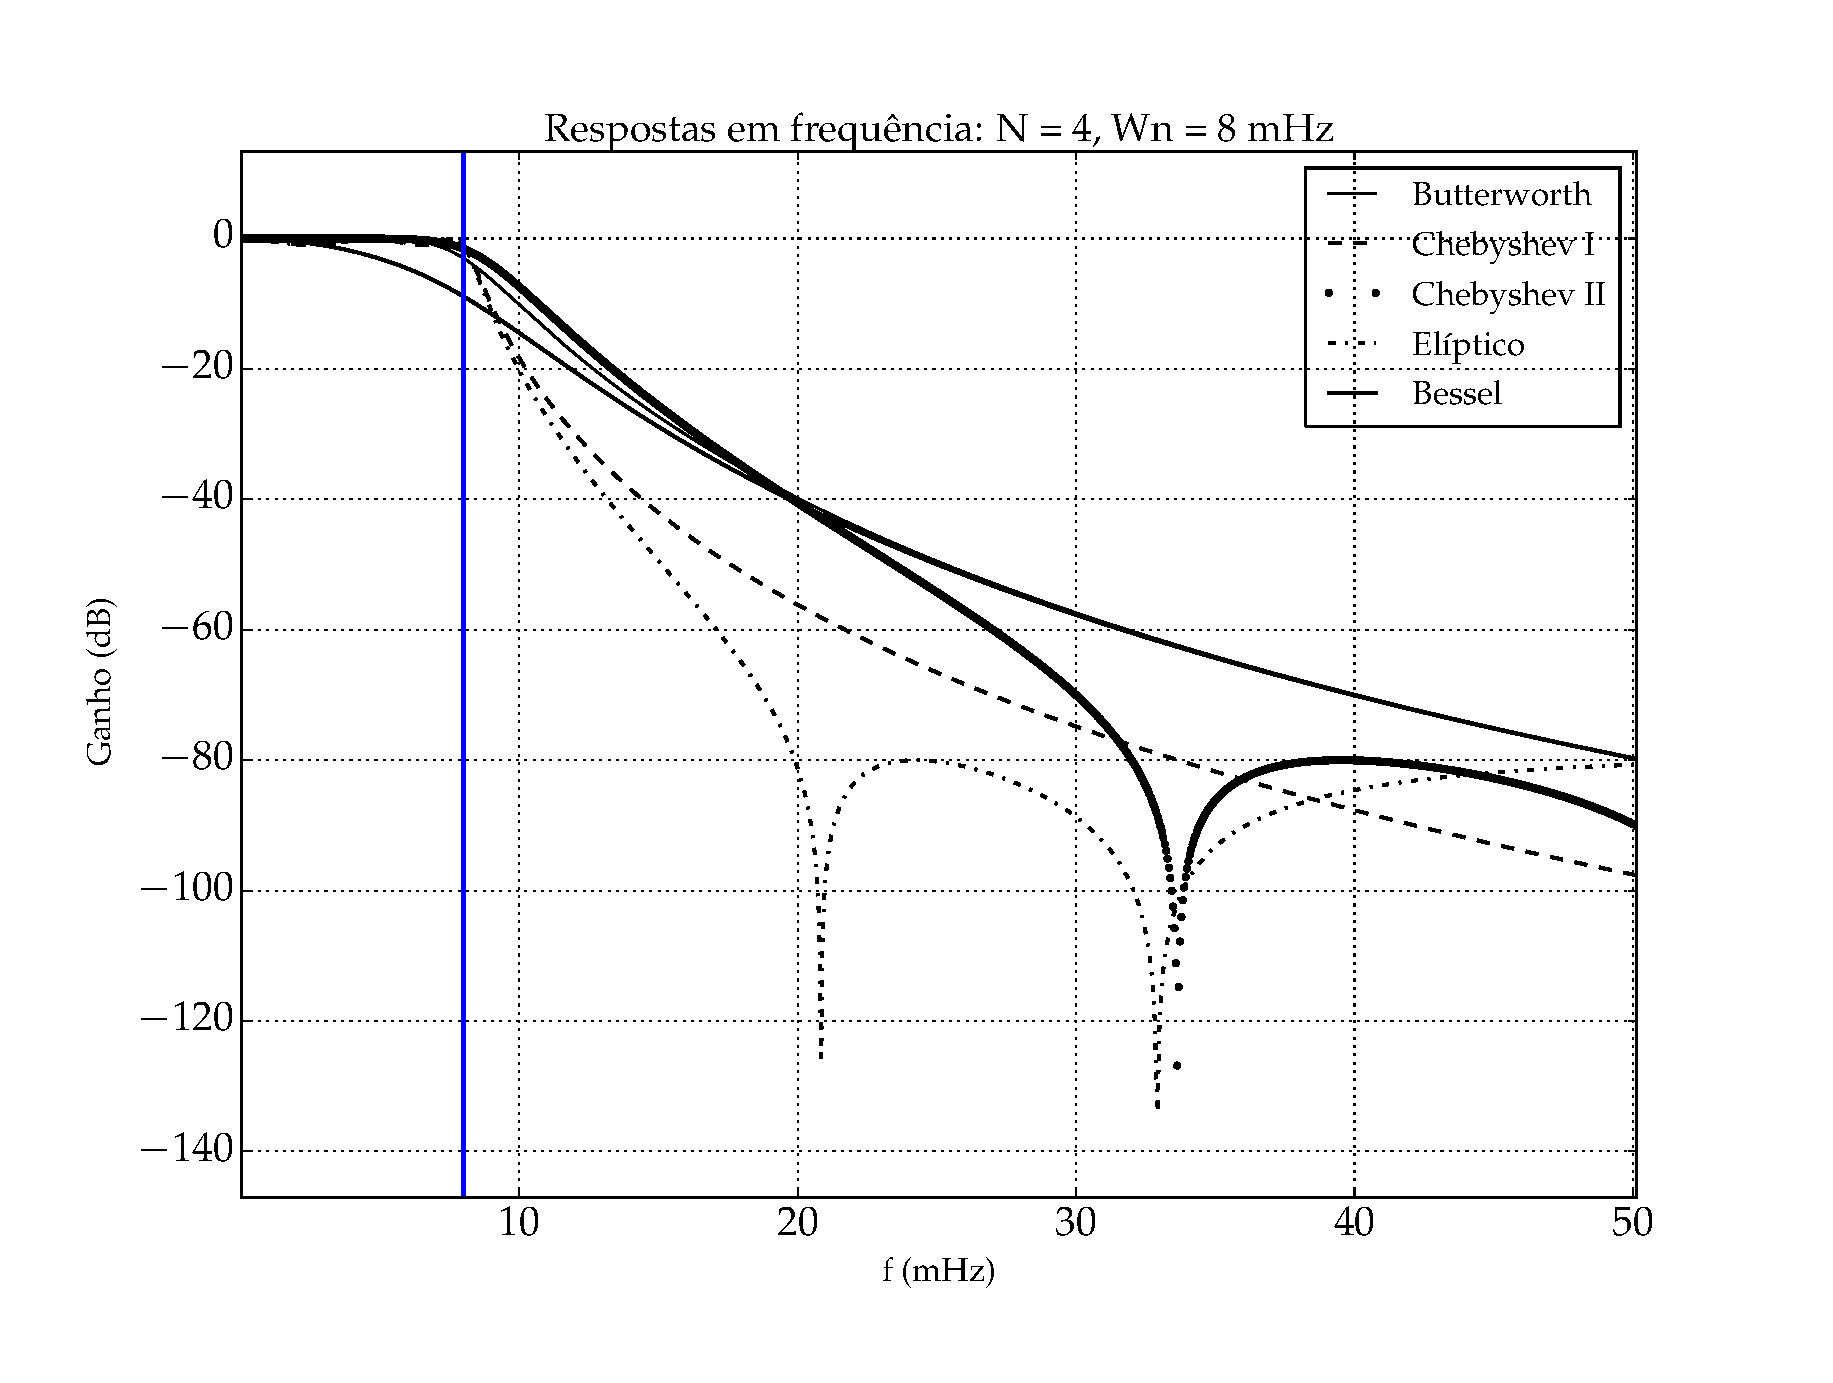
\includegraphics[scale=0.55]{images/plots/lowpass_IIR}
  \caption{Resposta em frequência para filtro low-pass IIR.}
  \label{fig:lowpass_iir_response}
\end{figure}

Constata-se que os resultados obtidos são muito próximos dos resultados do filtro analógico.

\subsection{Projeto Digital: FIR}
Como os filtros FIR são projetados de forma a aproximarem uma resposta em frequência ideal, especificou-se um filtro ideal passa-baixa com frequência de transição de 8 $mHz$; na banda de parada, definiu-se uma atenuação de 80 dB. Obteve-se:

\begin{figure}[H]
  \centering
  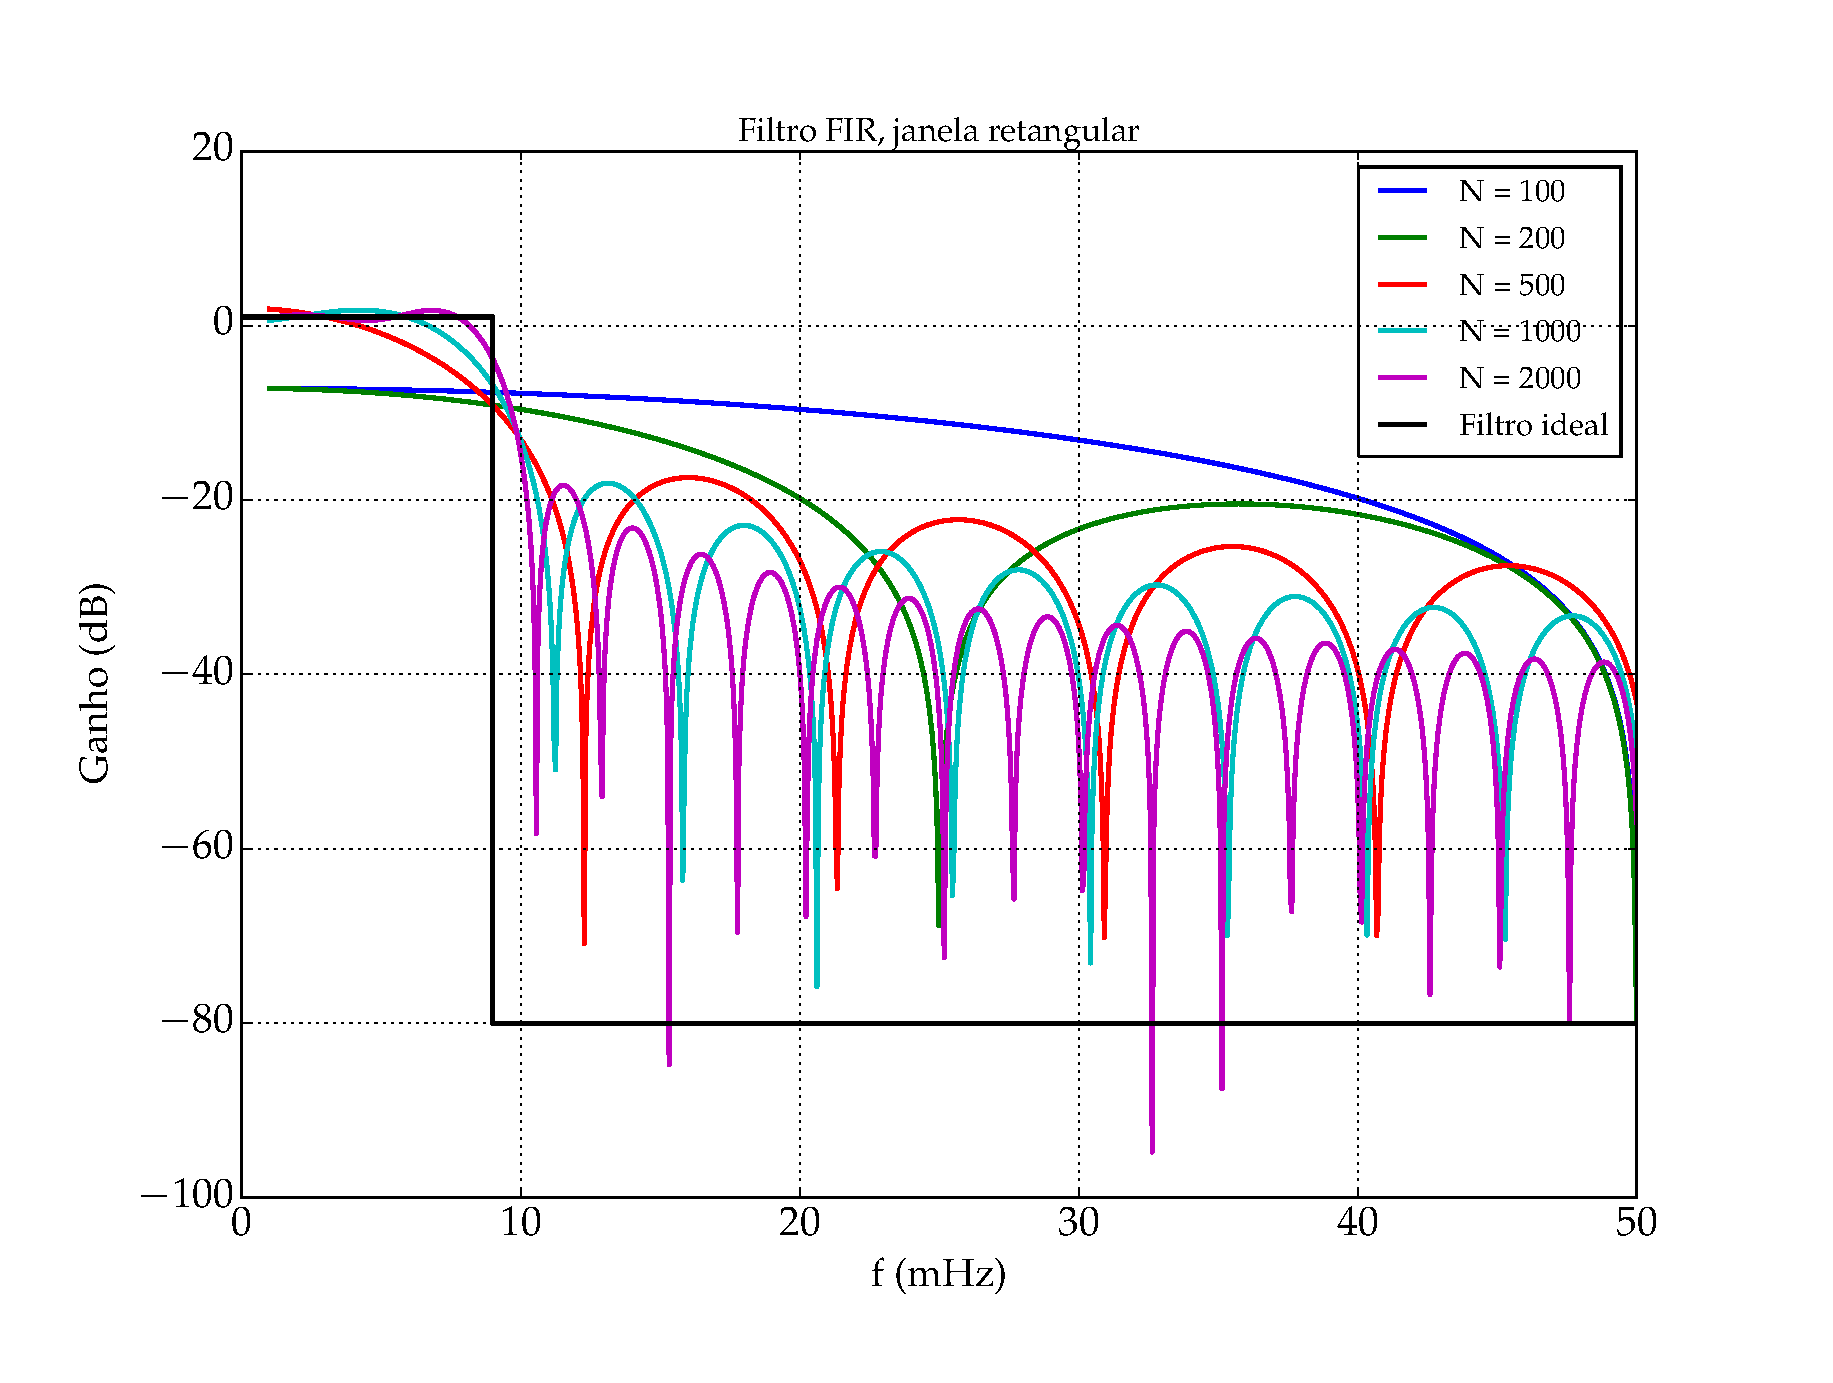
\includegraphics[scale=0.45]{images/plots/lowpass_FIR_rectangular_window}
  \caption{Resposta em frequência para filtro low-pass FIR com janela retangular.}
  \label{fig:lowpass_fir_rectang_response}
\end{figure}

\begin{figure}[H]
  \centering
  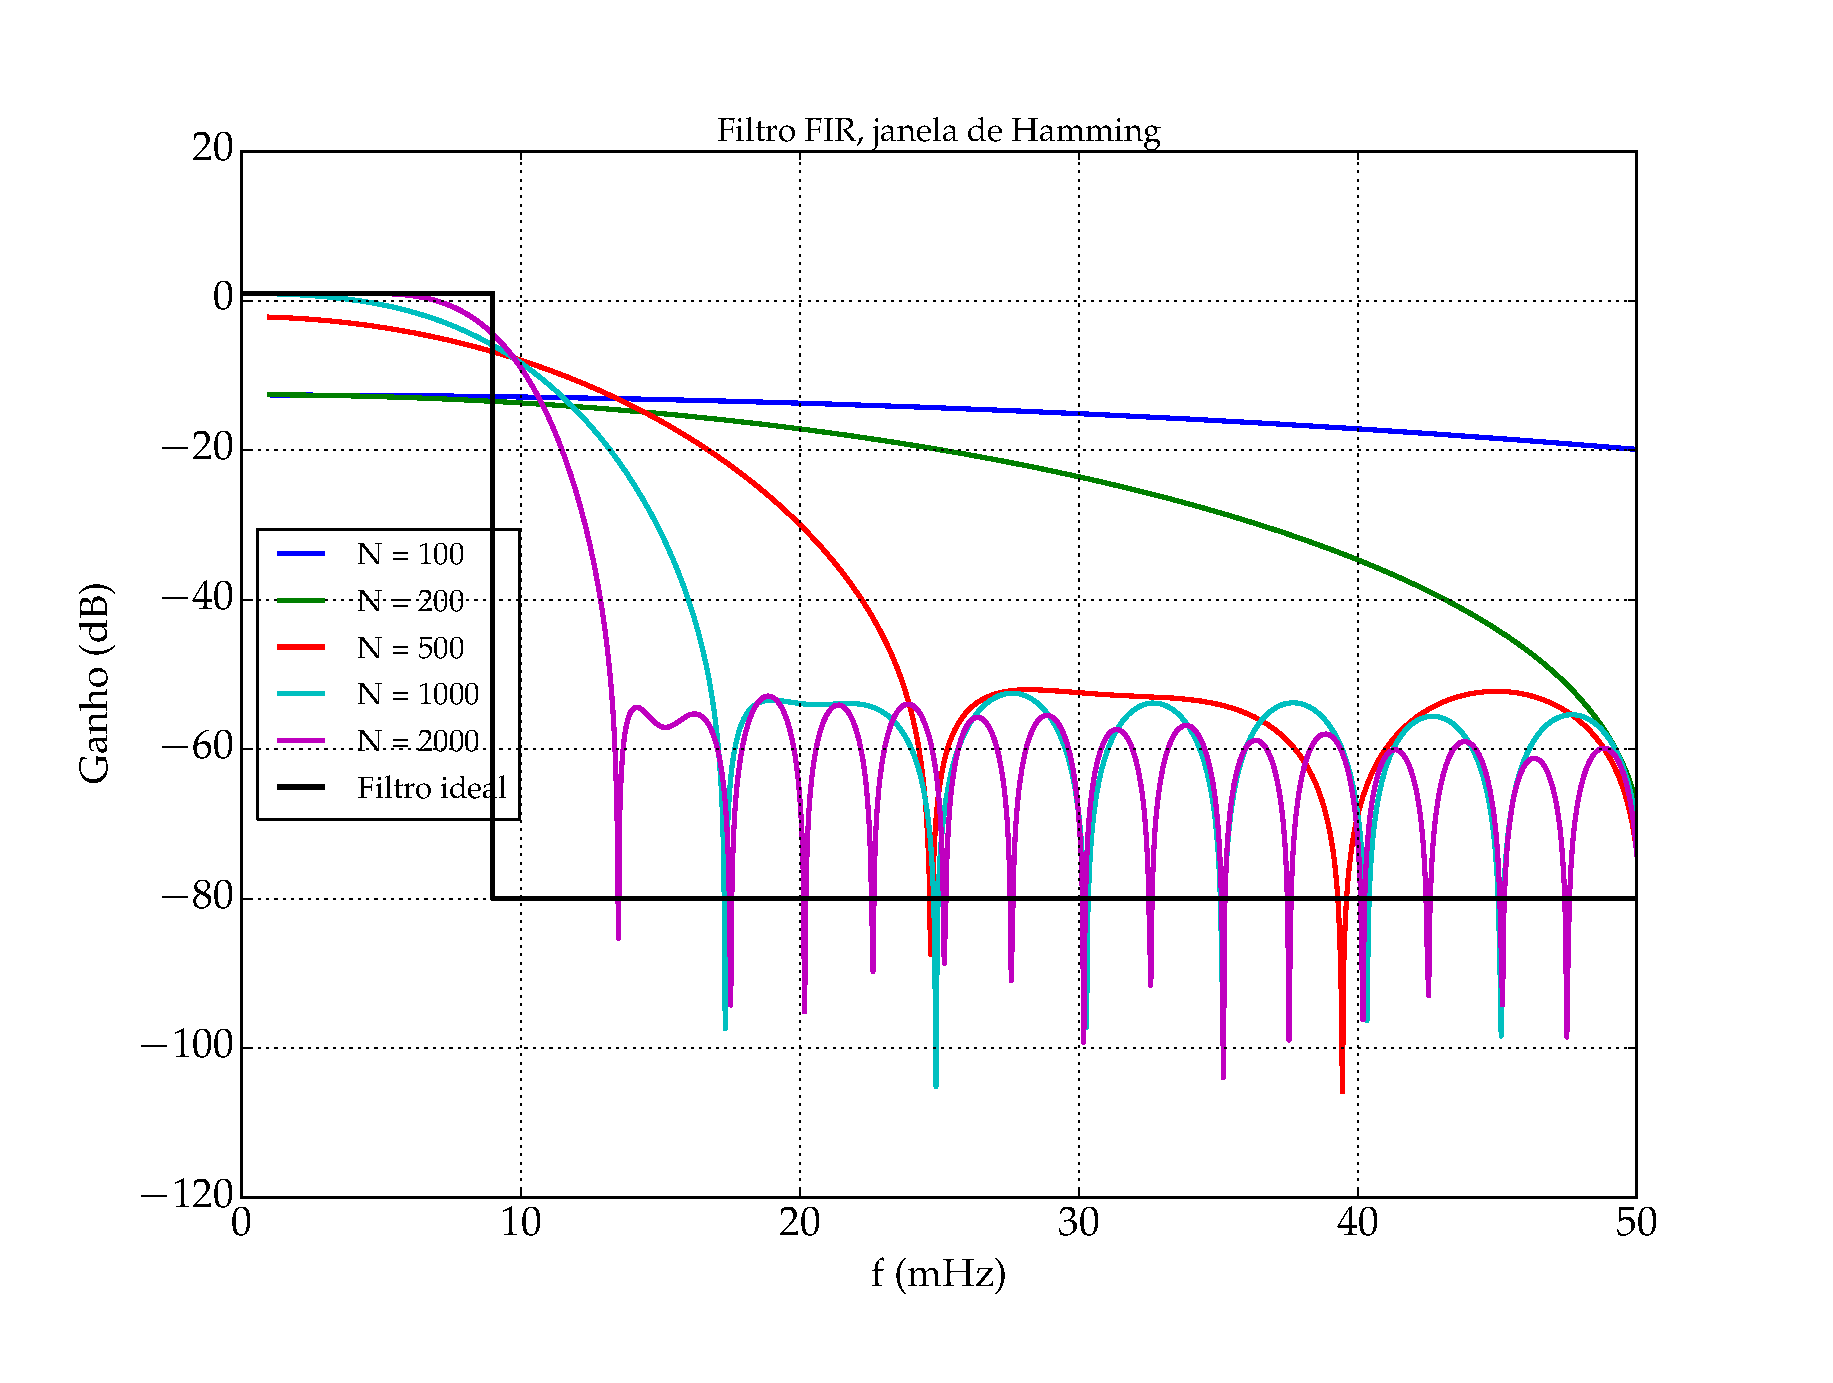
\includegraphics[scale=0.45]{images/plots/lowpass_FIR_hamming_window}
  \caption{Resposta em frequência para filtro low-pass FIR com janela de Hamming.}
  \label{fig:lowpass_fir_hamming_response}
\end{figure}

Verifica-se que, para ordens muito baixas, o filtro é incapaz de atender os requisitos especificados; já se esta for aumentada, os filtros apresentam maior proximidade daquele especificado, ao custo de maior \textit{ripple} na banda de parada.

A partir dos resultados apresentados nesta seção, pode-se afirmar que filtros digitais IIR são uma ferramenta possível para a filtragem de sinais de baixa frequência, devendo porém a taxa de amostragem ser compatível com a frequência dos sinais a serem processados.

\section{Exemplo de projeto: filtro \textit{notch}}
\label{sec:notch}
Uma aplicação bastante comum do projeto de filtros é o projeto de filtros \textit{notch} para remoção do ruído de 60 Hz da rede elétrica de um sinal. O filtro a ser projetado será um \textit{band-stop} cujas frequências de -3 dB são 59 e 61 Hz. 

Para o projeto dos filtros analógico e IIR definiu-se que o \textit{ripple} máximo aceitável é de 1 dB e que a atenuação na banda de parada será de 80 dB.

\subsection{Projeto Analógico}
Na figura \ref{fig:bandstop_analog_response} apresentam-se as respostas em frequência de um filtro \textit{band-stop} de 5\textsuperscript{a} ordem, nas frequências de corte especificadas anteriormente, para diferentes funções de transferência:

\begin{figure}[H]
  \centering
  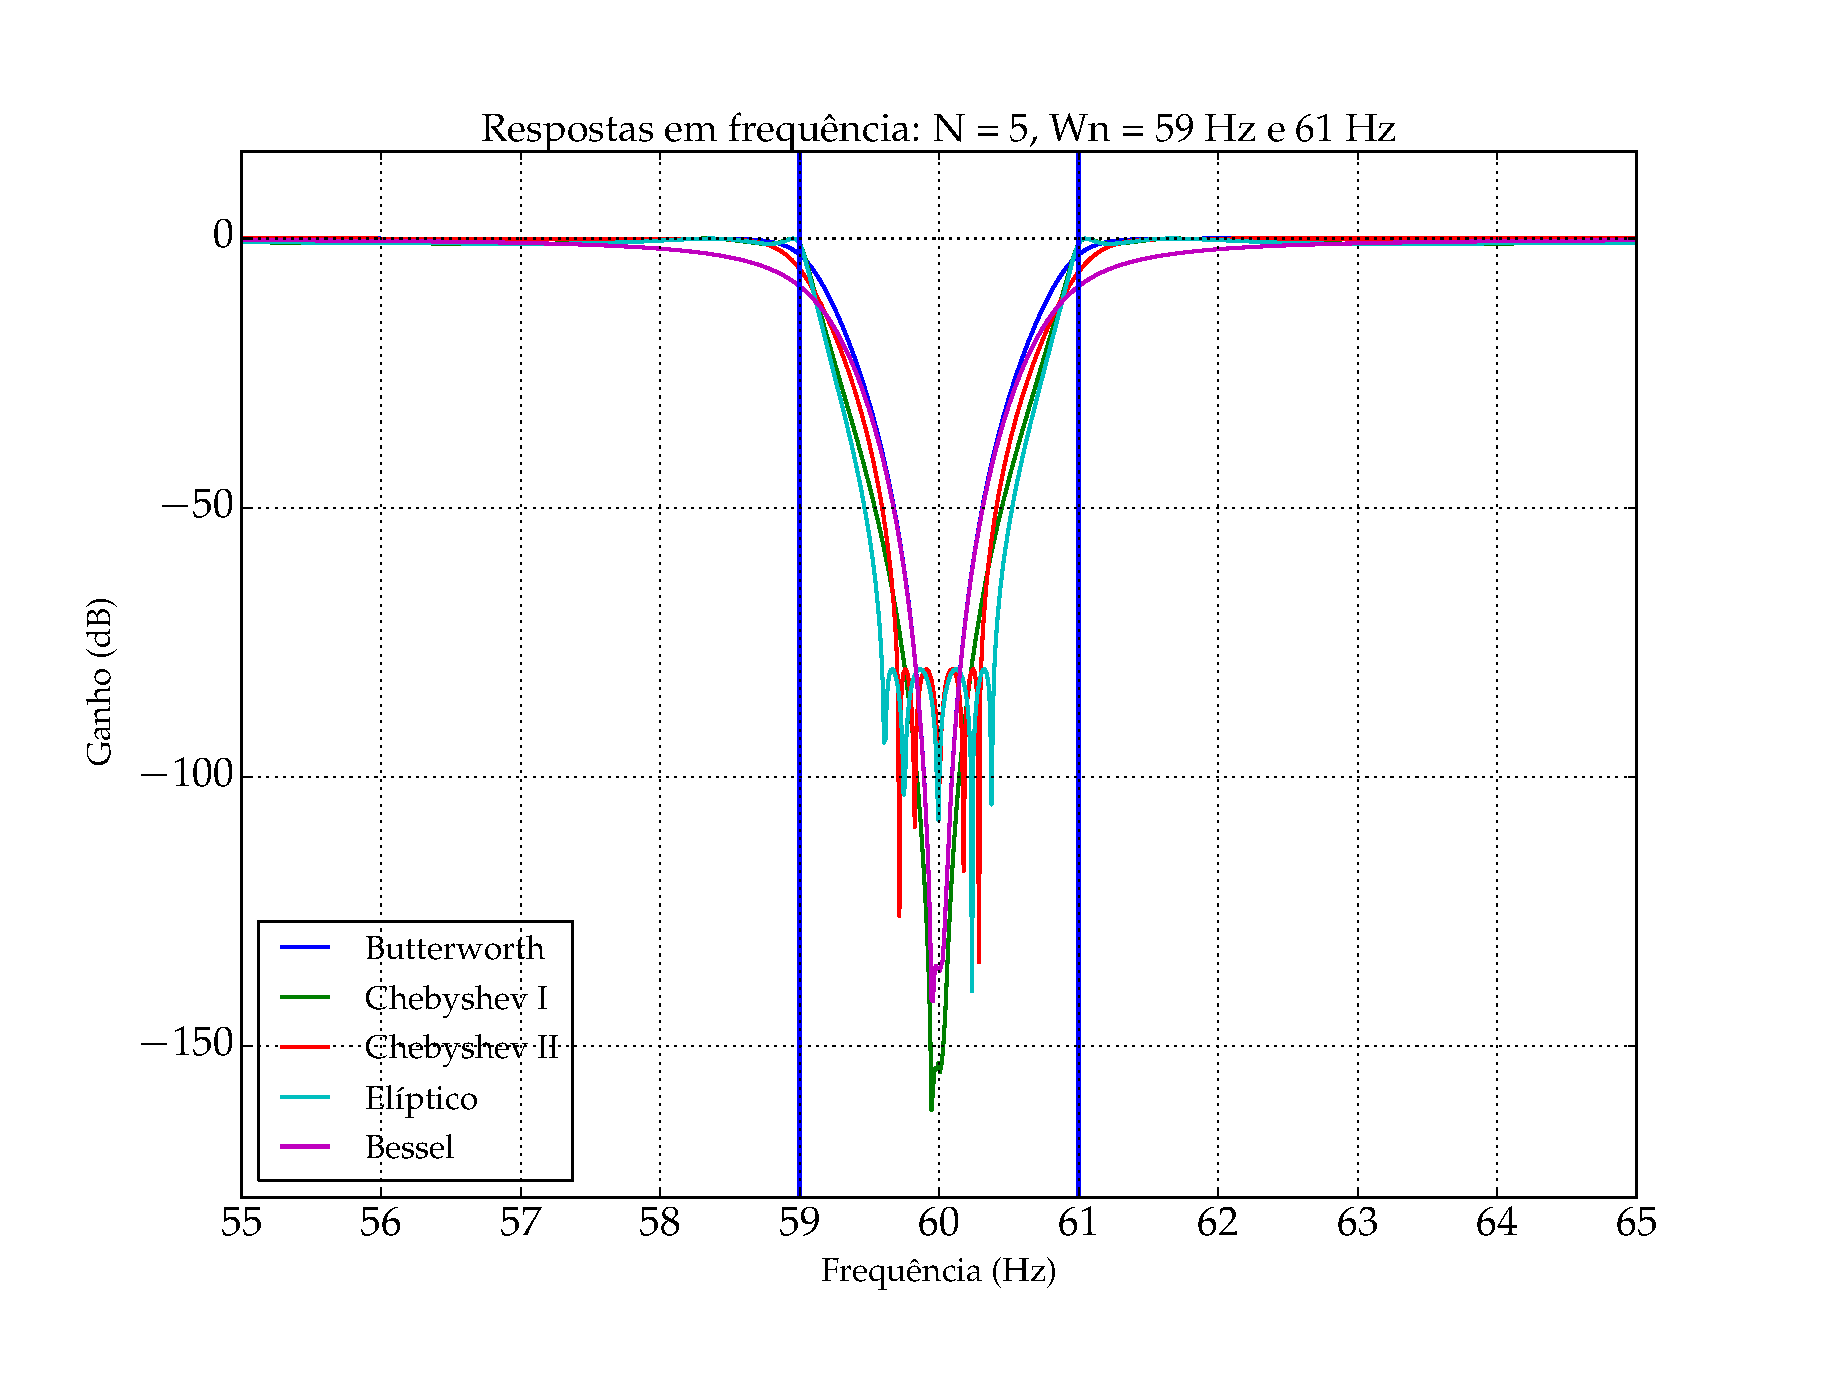
\includegraphics[scale=0.48]{images/plots/bandstop_analog}
  \caption{Resposta em frequência para filtro band-stop analógico.}
  \label{fig:bandstop_analog_response}
\end{figure}

Verifica-se o comportamento descrito na revisão teórica do presente trabalho, sendo que no filtro Chebyshev tipo II, a(s) frequência(s) $\omega_n$ representam os pontos nos quais é atingida a atenuação na banda de parada (ao contrário dos outros filtros, onde elas representam as frequências de $-3$ dB).

\subsection{Projeto Digital: IIR}
Projetou-se um filtro com especificações similares ao do analógico apresentado anteriormente, sendo a frequência de amostragem definida em 1000 Hz. Obteve-se a seguinte resposta em frequência:

\begin{figure}[H]
  \centering
  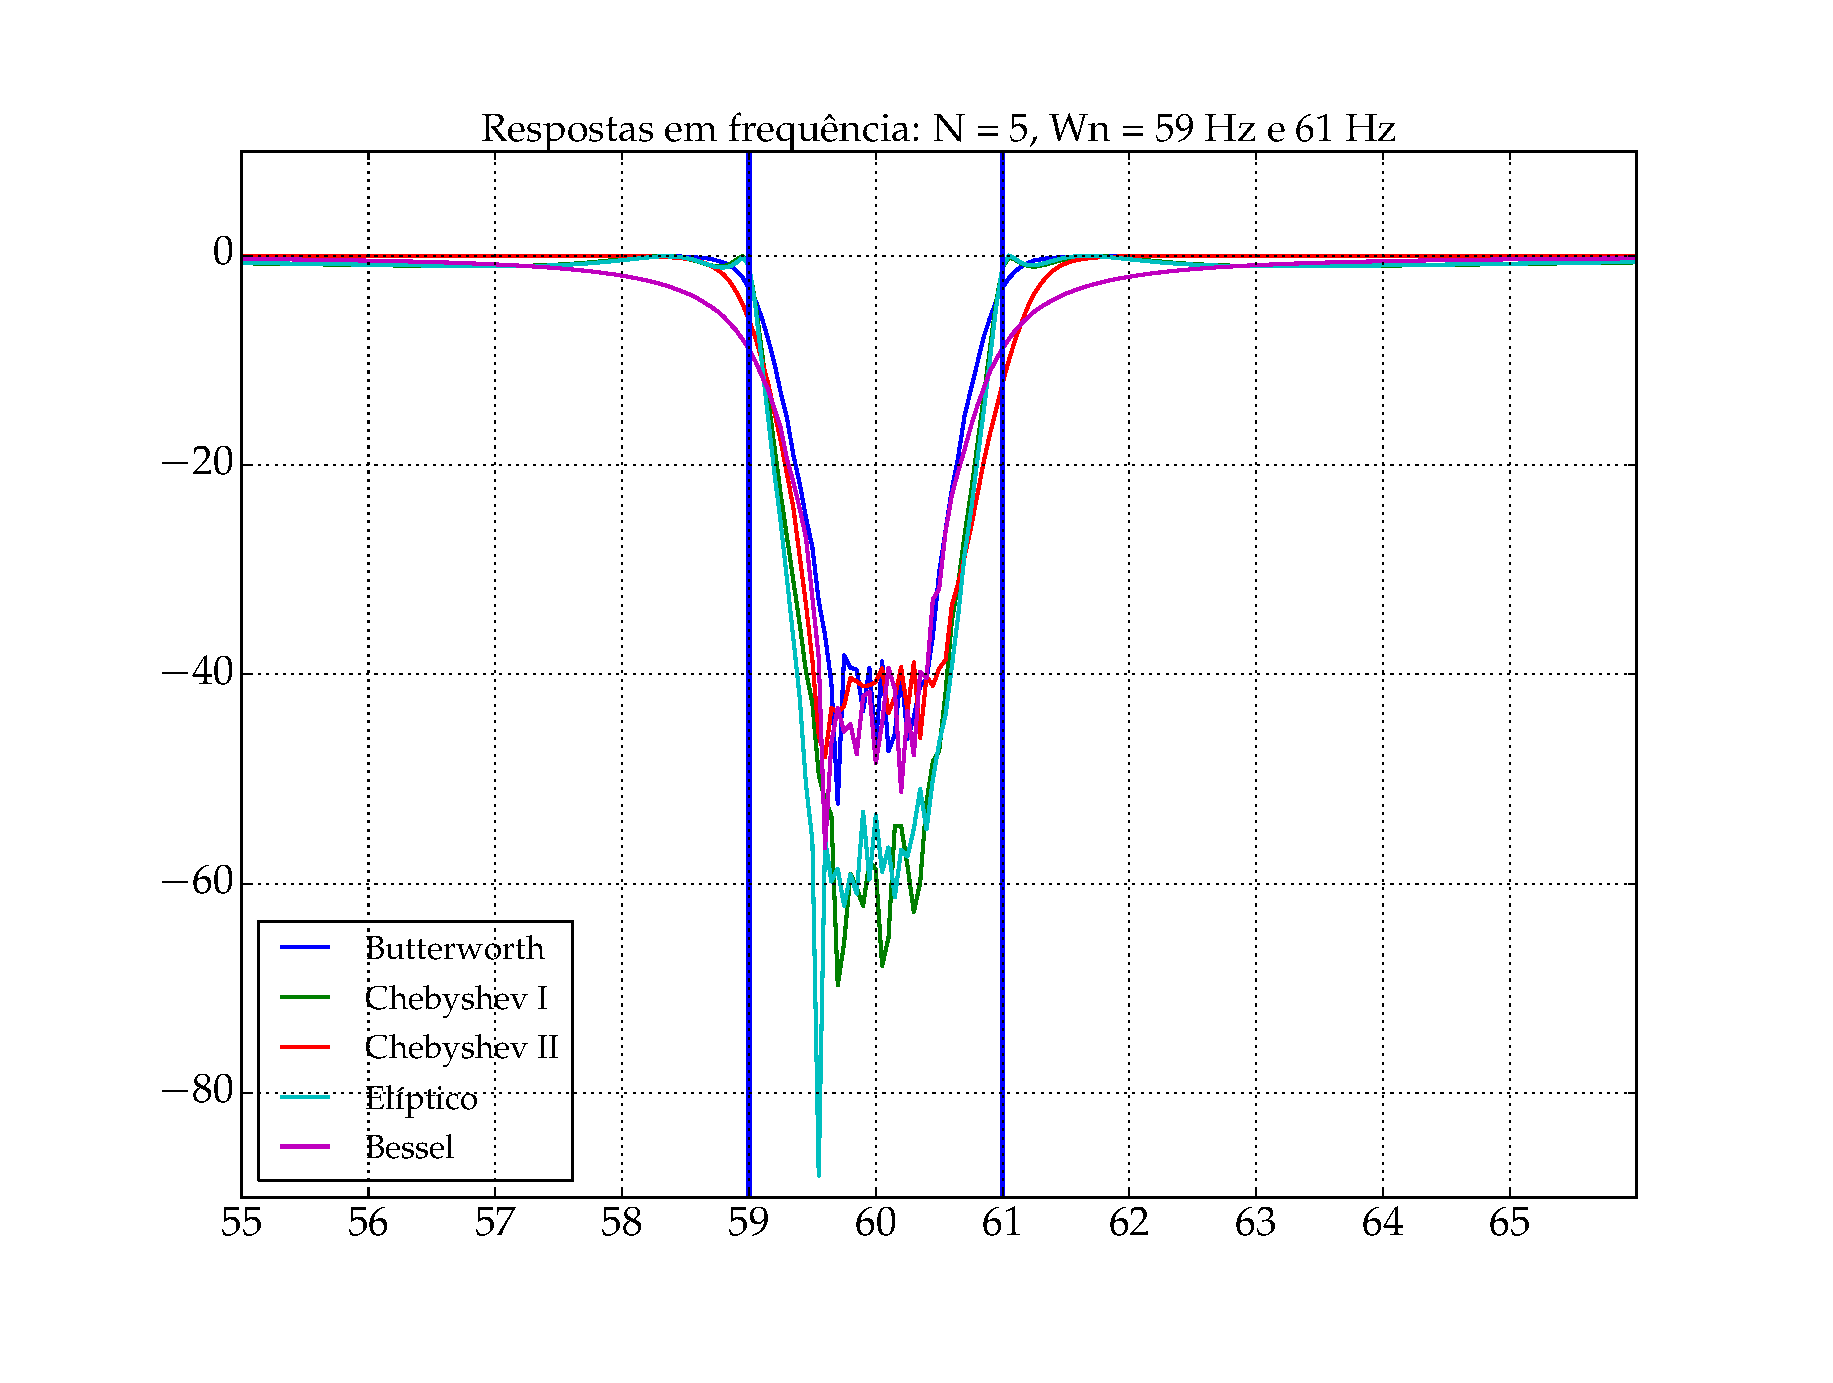
\includegraphics[scale=0.55]{images/plots/bandstop_IIR}
  \caption{Resposta em frequência para filtro band-stop IIR.}
  \label{fig:bandstop_IIR_response}
\end{figure}

As mesmas conclusões feitas no item anterior para os filtros analógicos podem ser feitas aqui; todavia, constata-se a presença de pequenas e praticamente desprezíveis oscilações devido ao processo de discretização.

\newpage
\subsection{Projeto Digital: FIR}
O projeto deste filtro é especificado em função de ganhos e bandas; dessa forma, define-se:

\begin{itemize}
\item{\textbf{Banda de passagem}}: 0-58 Hz e 61-500 Hz, com ganho de 0 dB;
\item{\textbf{Banda de parada}}: 59-61 Hz, com atenuação de 80 dB.
\end{itemize}

Foram obtidos os seguintes resultados para diferentes números $N$ de \textit{taps}\footnote{Não há uma regra geral para estimar a ordem necessária; desta forma, o processo muitas vezes envolve a simulação com diferentes ordens até atingida a resposta desejada}, quando empregada a função janela retangular:

\begin{figure}[H]
  \centering
  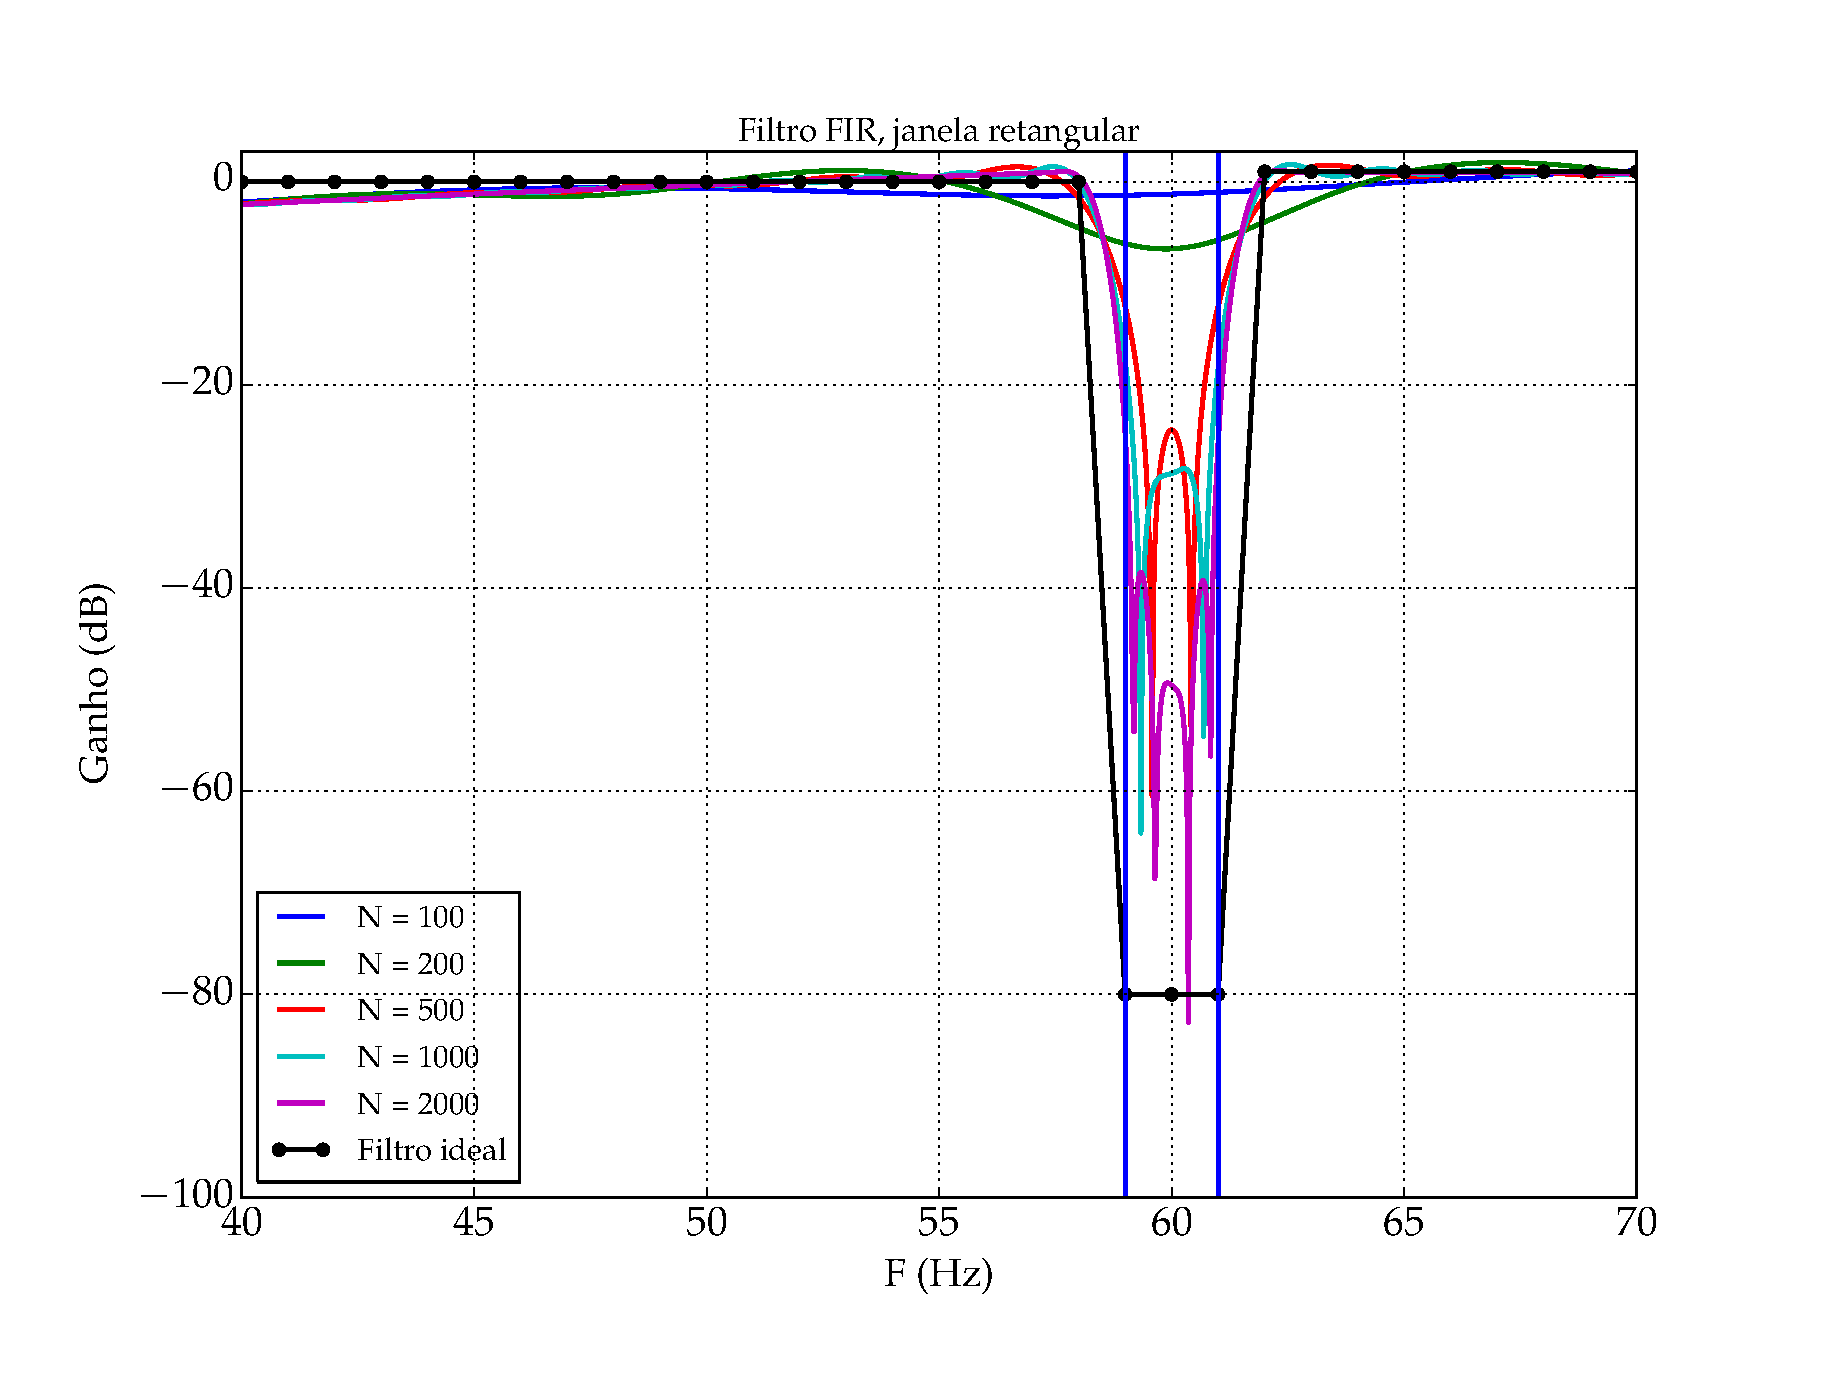
\includegraphics[scale=0.55]{images/plots/bandstop_FIR_rectangular_window}
  \caption{Resposta em frequência para filtro band-stop FIR com a função janela retangular.}
  \label{fig:bandstop_FIR_rectangular}
\end{figure}

\newpage
Quando é empregada a função janela de Hamming, tem-se o seguinte resultado:

\begin{figure}[H]
  \centering
  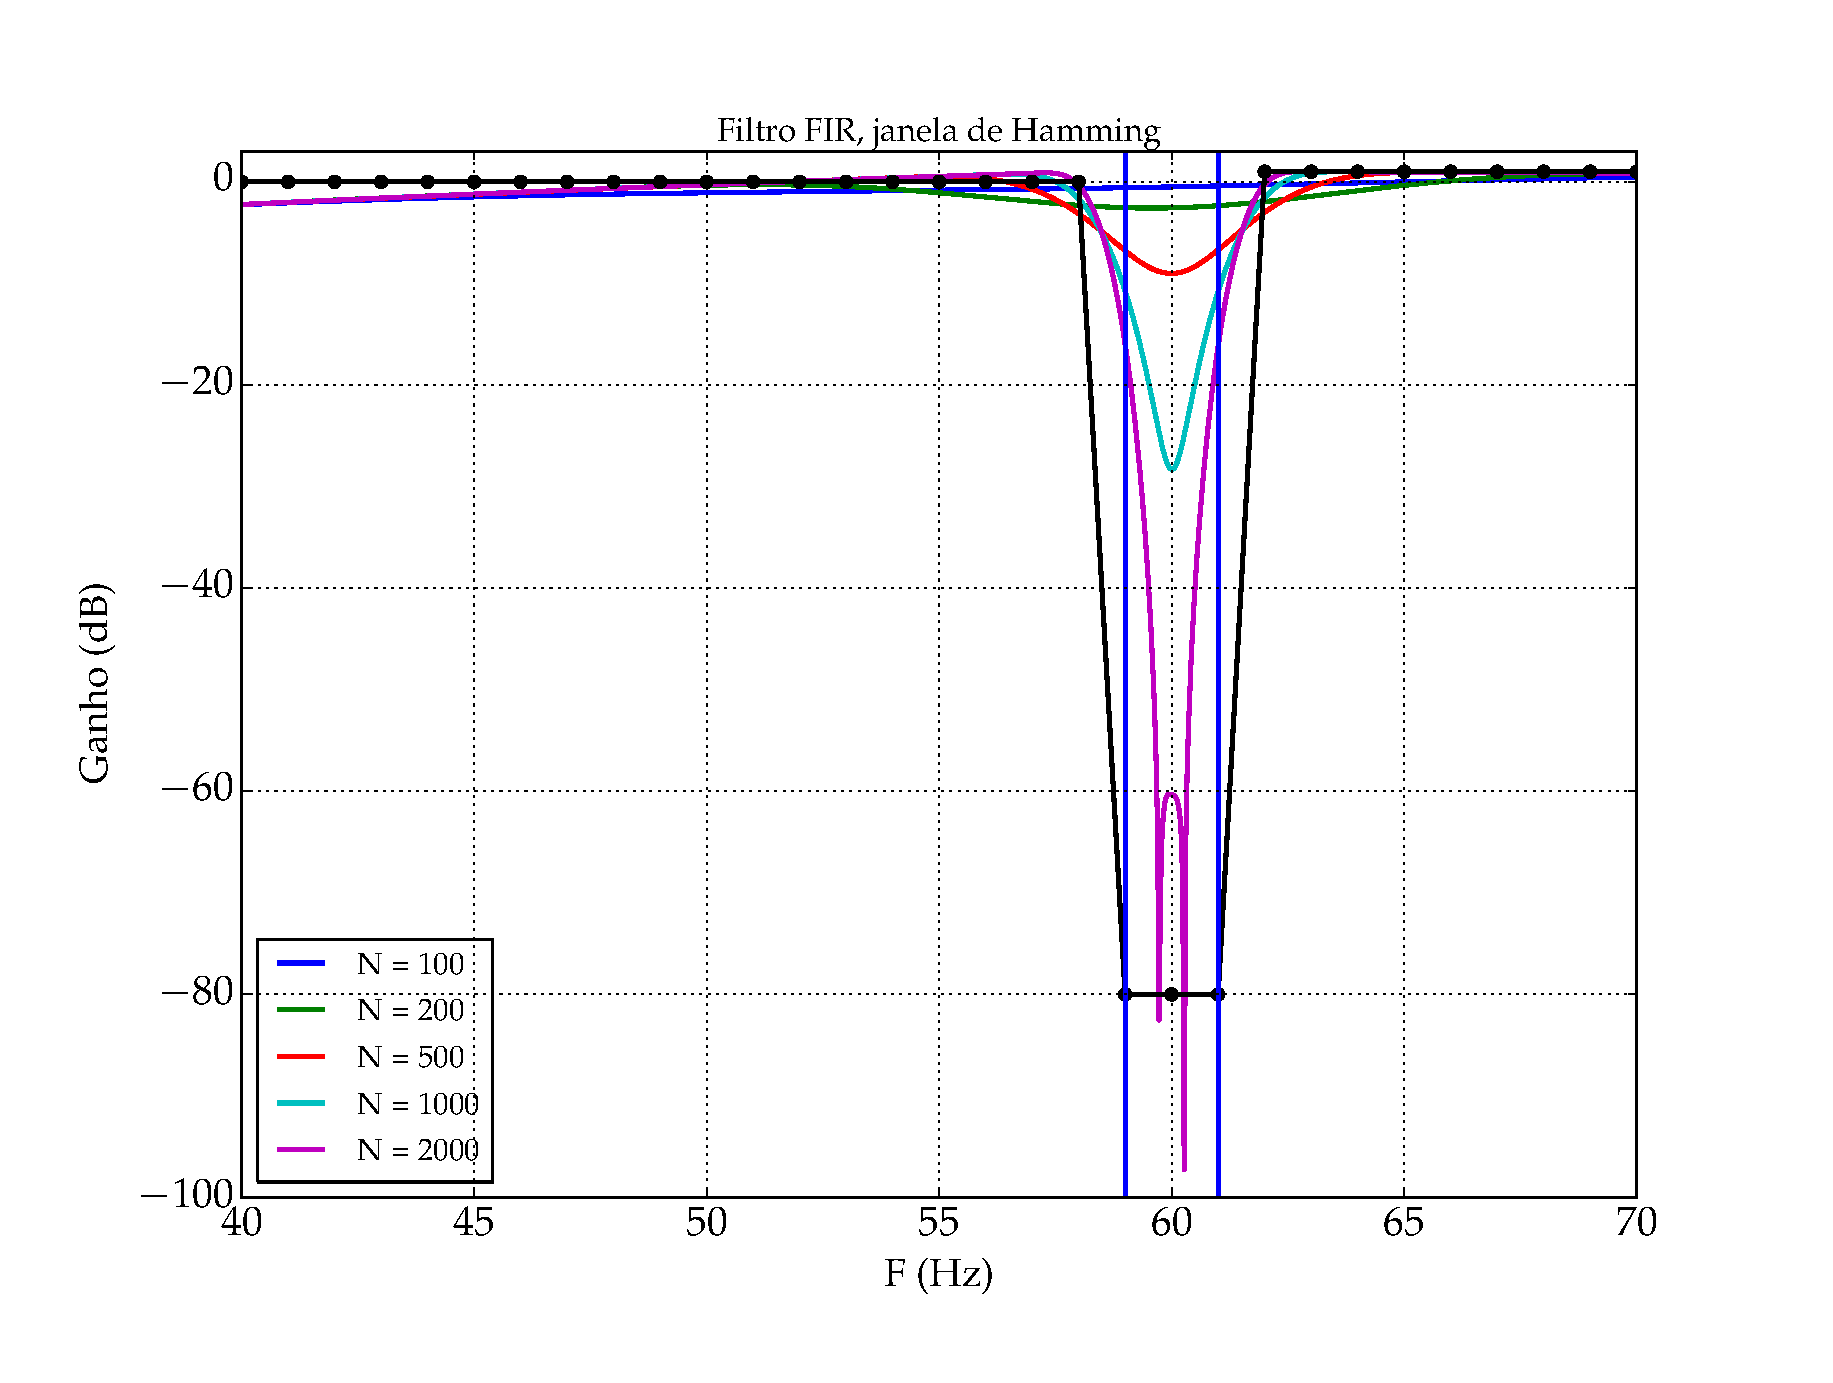
\includegraphics[scale=0.55]{images/plots/bandstop_FIR_hamming_window}
  \caption{Resposta em frequência para filtro band-stop FIR com a função janela de Hamming.}
  \label{fig:bandstop_FIR_hamming}
\end{figure}

\newpage

Já para a janela triangular, tem-se:

\begin{figure}[H]
  \centering
  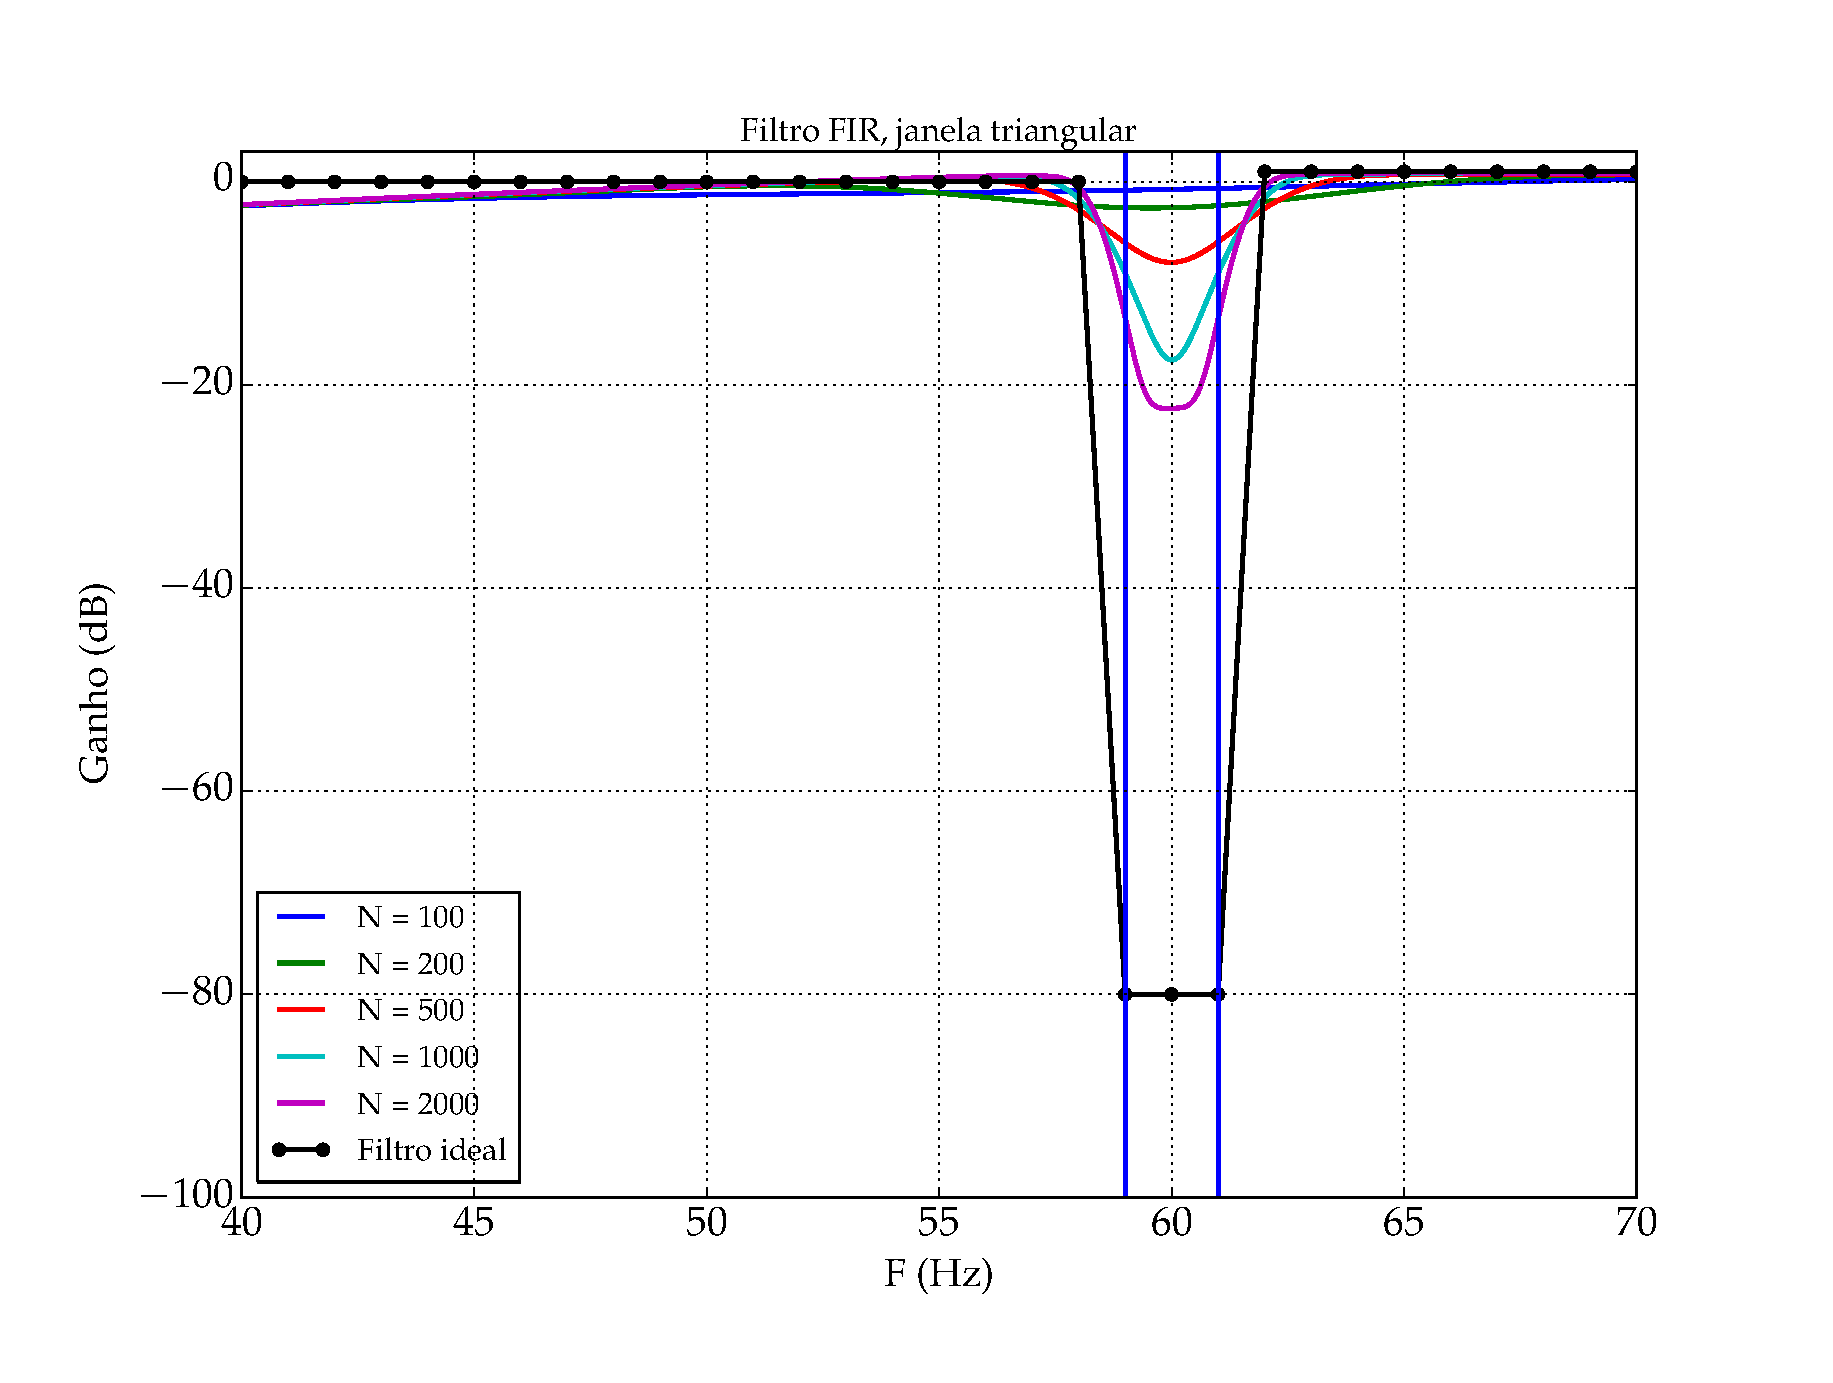
\includegraphics[scale=0.55]{images/plots/bandstop_FIR_triang_window}
  \caption{Resposta em frequência para filtro band-stop FIR com a função janela  triangular.}
  \label{fig:bandstop_FIR_triangular}
\end{figure}

De imediato constata-se que, para atingir o mesmo desempenho dos filtros IIR, é necessário um número maior de iterações. Verifica-se que as funções janela de Hamming e triangular não tem o \textit{ripple} na banda de parada, ao custo de apresentarem uma menor atenuação - e também pode ser visto que a função janela triangular é inadequada para a aplicação proposta. A função janela retangular, também, atinge um resultado mais próximo dos filtros IIR elíptico e Chebyshev tipo II.

\newpage

Para o filtro \textit{equirripple} sintetizado pelo algoritmo de Parks-McClellan, é obtido: 

\begin{figure}[H]
  \centering
  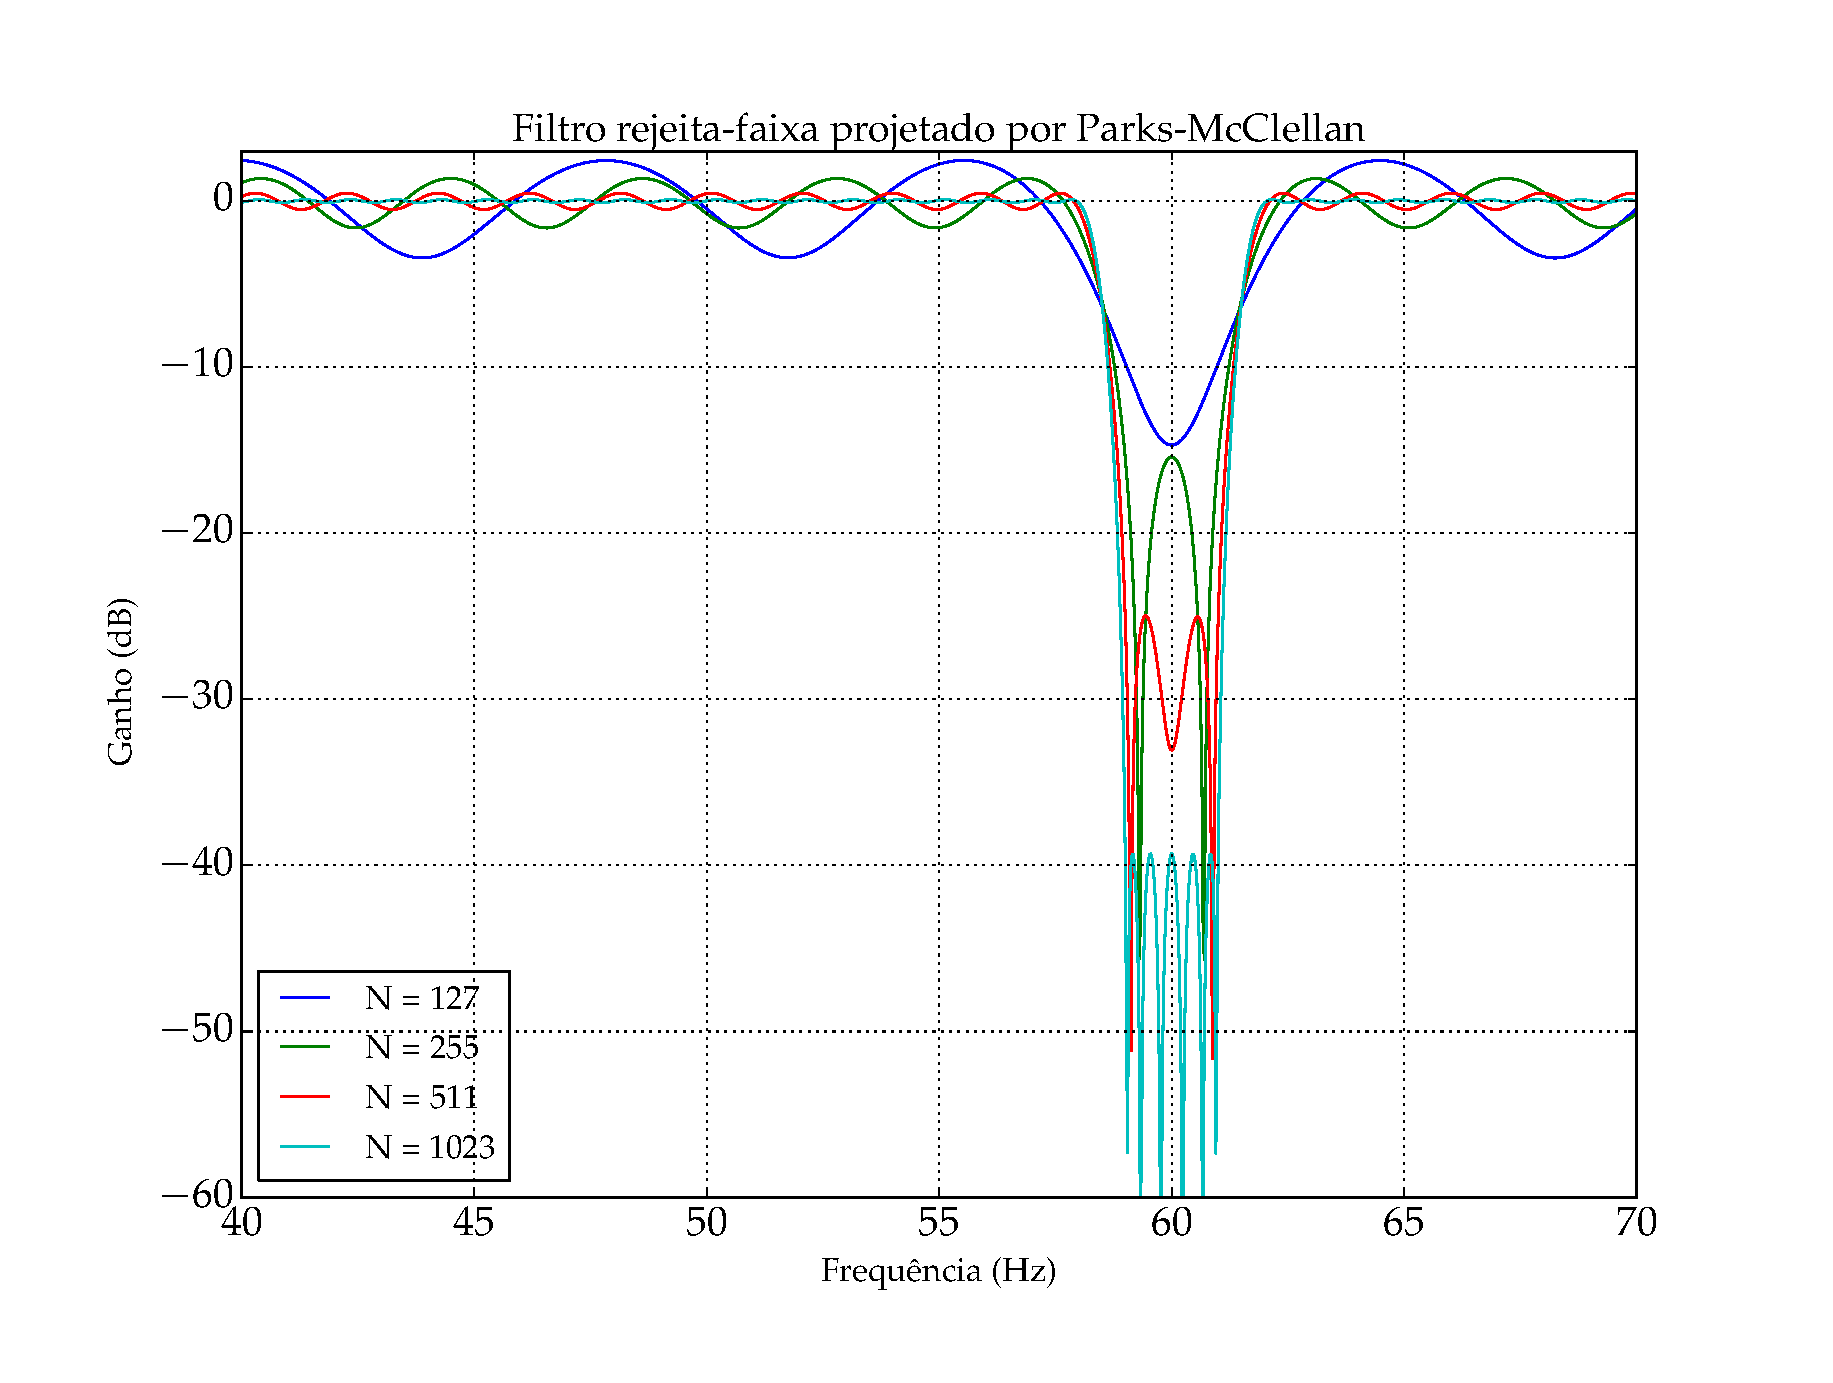
\includegraphics[scale=0.55]{images/plots/bandstop_fir_pm}
  \caption{Resposta em frequência para filtro band-stop FIR projetado pelo algoritmo de Parks-McClellan.}
  \label{fig:bandstop_FIR_pm}
\end{figure}

Para o filtro implementado por esse algoritmo, tem-se uma imposição do algoritmo que requer que filtros \textit{bandstop} tenham ordem ímpar, caso contrário os objetivos não são atingidos.

Pode-se verificar que esta família de filtros apresenta o \textit{ripple} igual para todas as frequências na banda de passagem,  sendo que este é inversamente proporcional à ordem do filtro ao custo de oscilações na banda de parada.

\newpage
\section{Exemplo de projeto: filtro passa-banda}
\label{sec:bandpass}
Em aplicações de áudio e de telefonia é bastante comum a necessidade de filtros para permitir a passagem da voz humana, na faixa de 300 a 4000 Hz. Para este projeto tem-se as seguintes especificações:

\begin{itemize}
\item \textbf{Bandas de parada}: 100-300 Hz e 4000-6000 Hz.
\item \textbf{Banda de passagem}: 300 a 4000 Hz
\item \textbf{Ripple na banda de passagem}: 3 dB
\item \textbf{Atenuação na banda de parada}: 80 dB
\end{itemize}

e devem-se determinar ordem e frequências críticas que as satisfaçam.

\subsection{Projeto Analógico}

\begin{figure}[H]
  \centering
  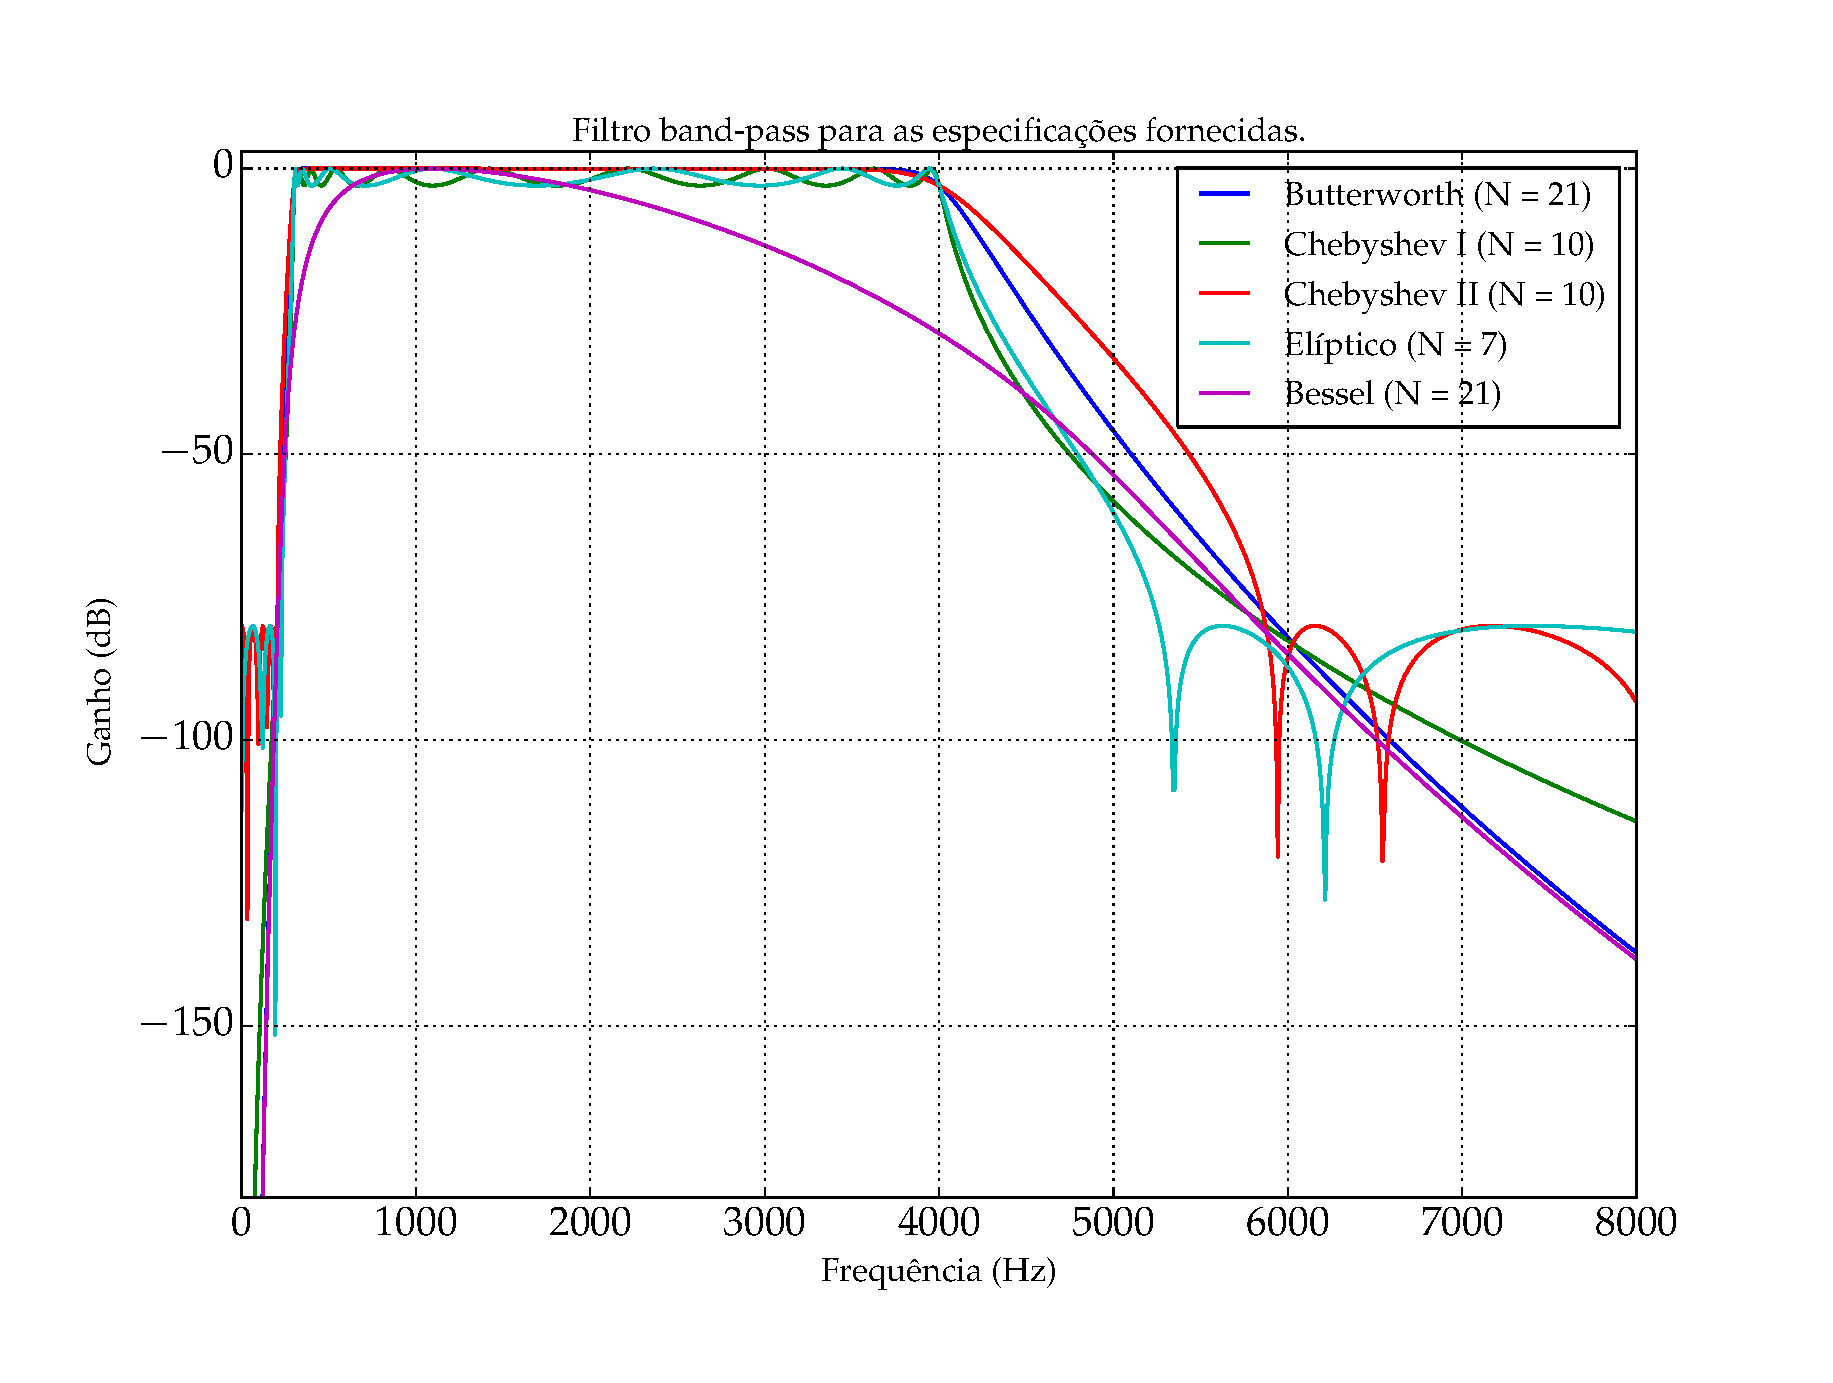
\includegraphics[scale=0.55]{images/plots/bandpass_analog}
  \caption{Resposta em frequência para filtro band-pass analógico.}
  \label{fig:bandpass_analog}
\end{figure}

A partir desses resultados, os \textit{trade-offs} entre os diferentes tipos de filtros ficam claros. Verifica-se que o filtro de Butterworth, embora não apresente \textit{ripple}, precisa de maior ordem para atingir resultados similares aos outros filtros; já o filtro de Bessel demonstrou-se insuficiente para atingir a especificação solicitada. O filtro elíptico consegue fornecer, para uma menor ordem, resultados bastante similares às outras topologias.

Um dos problemas já citados anteriormente e que foi constatado nesse exemplo de projeto foram instabilidades numéricas: inicialmente foi tentado o projeto com uma especificação de banda de parada de 4000 a 5000 Hz, porém os algoritmos falhavam ao calcular a resposta em frequência. O MATLAB tenta contornar esse problema calculando o filtro em seções de segunda ordem (\textit{second order sections}), as quais não foram implementadas em Python, ficando em aberto a ideia de sua implementação.

\subsection{Projeto Digital: IIR}
Para este projeto, foi estabelecida uma taxa de amostragem de 20 KHz.

\begin{figure}[H]
  \centering
  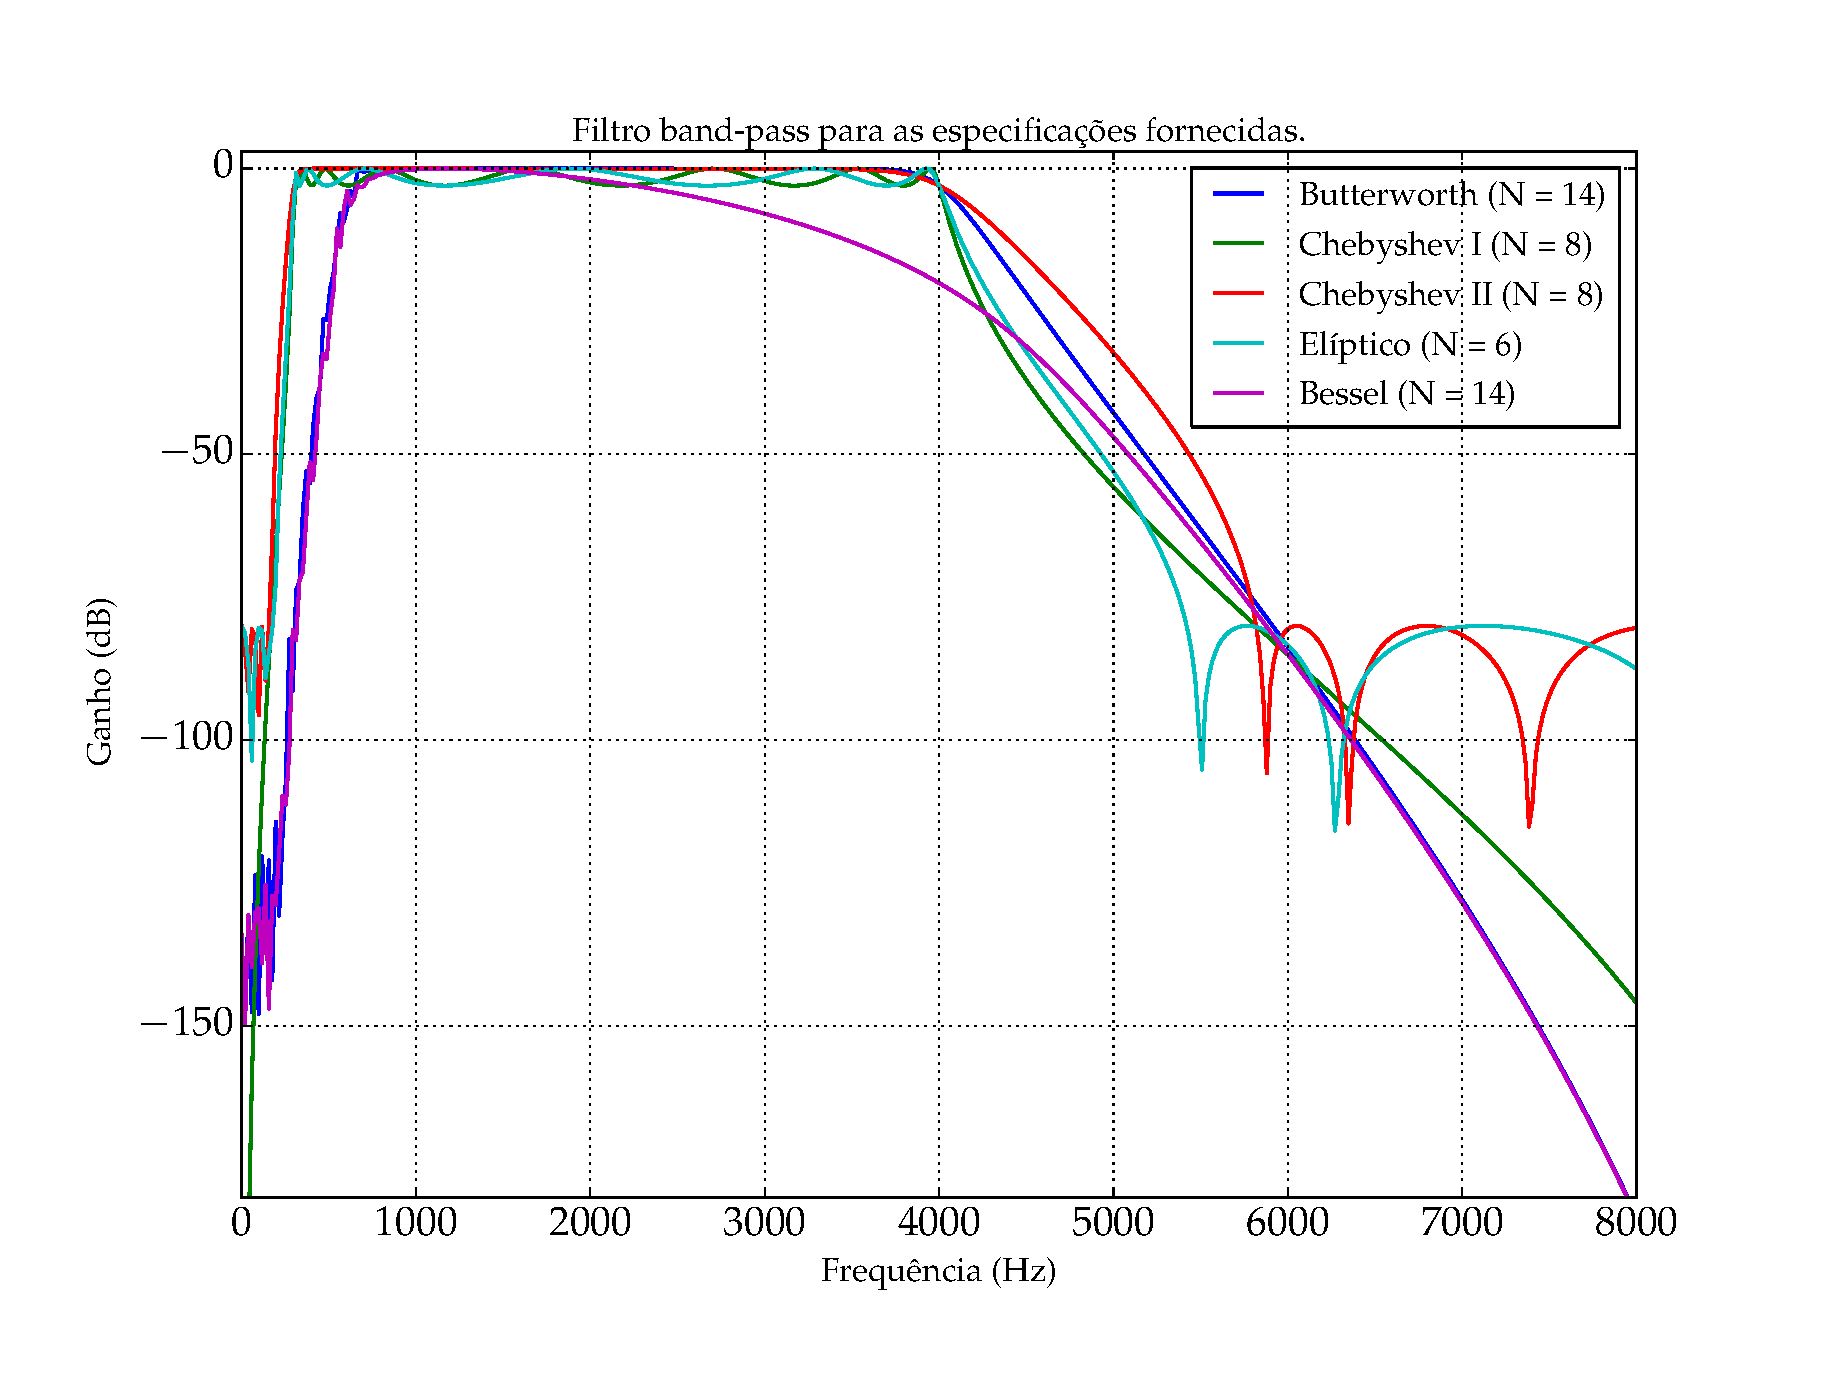
\includegraphics[scale=0.5]{images/plots/bandpass_IIR}
  \caption{Resposta em frequência para filtro band-pass IIR.}
  \label{fig:bandpass_IIR}
\end{figure}

Os resultados de ambos projetos são bem similares, valendo as mesmas conclusões que foram feitas para o projeto analógico.

\subsection{Projeto Digital: FIR}

Foi especificado um filtro ideal, com 0 dB de ganho na faixa de 300 a 4000 Hz e -80 dB fora dela, tendo-se obtido: 

\begin{figure}[H]
  \centering
  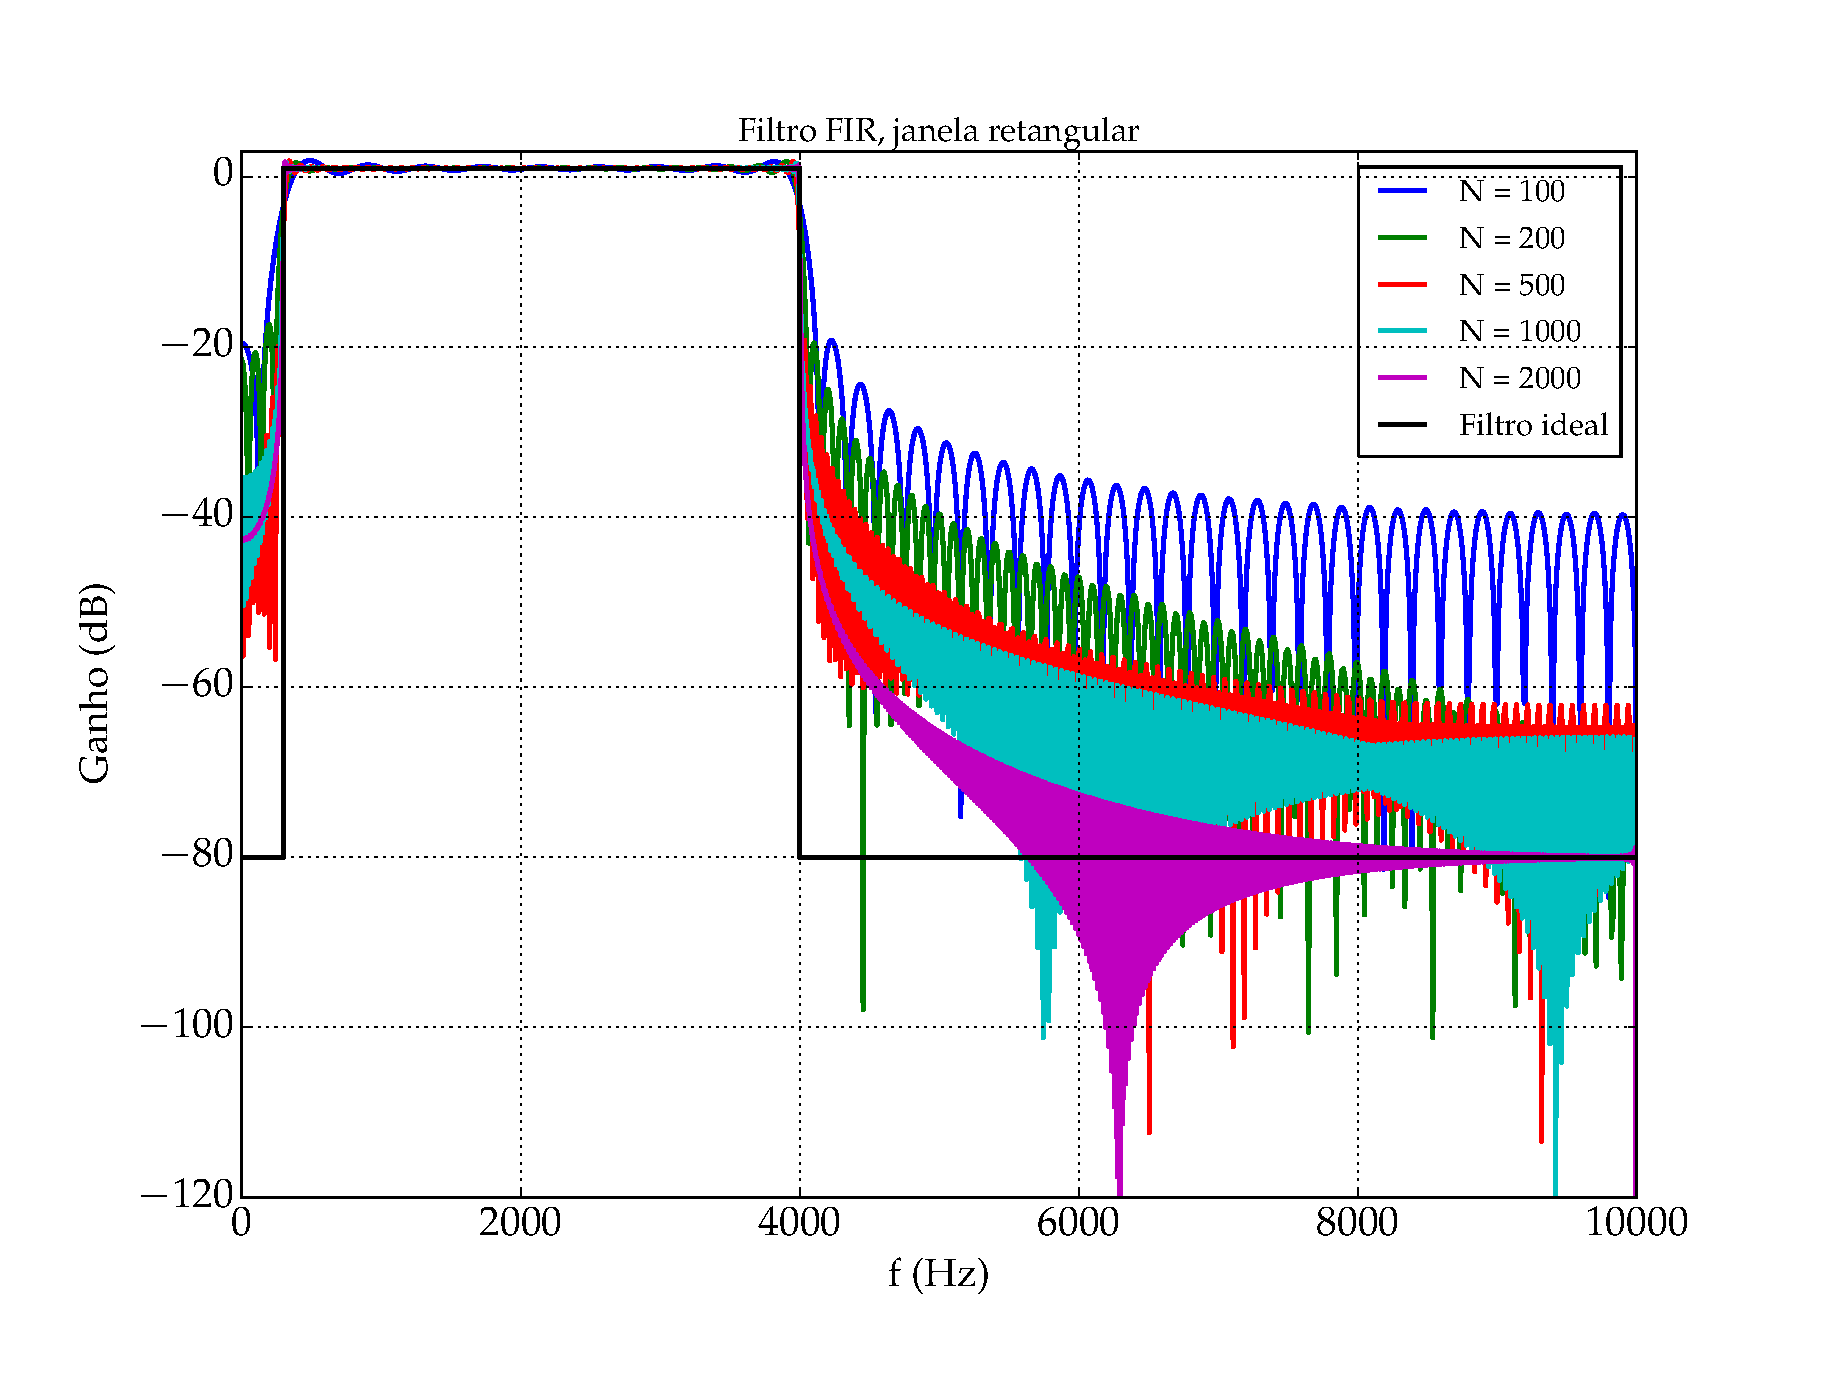
\includegraphics[scale=0.55]{images/plots/bandpass_FIR_rectangular_window}
  \caption{Resposta em frequência para filtro band-pass FIR com a função janela retangular.}
  \label{fig:bandpass_FIR_rectangular}
\end{figure}

\begin{figure}[H]
  \centering
  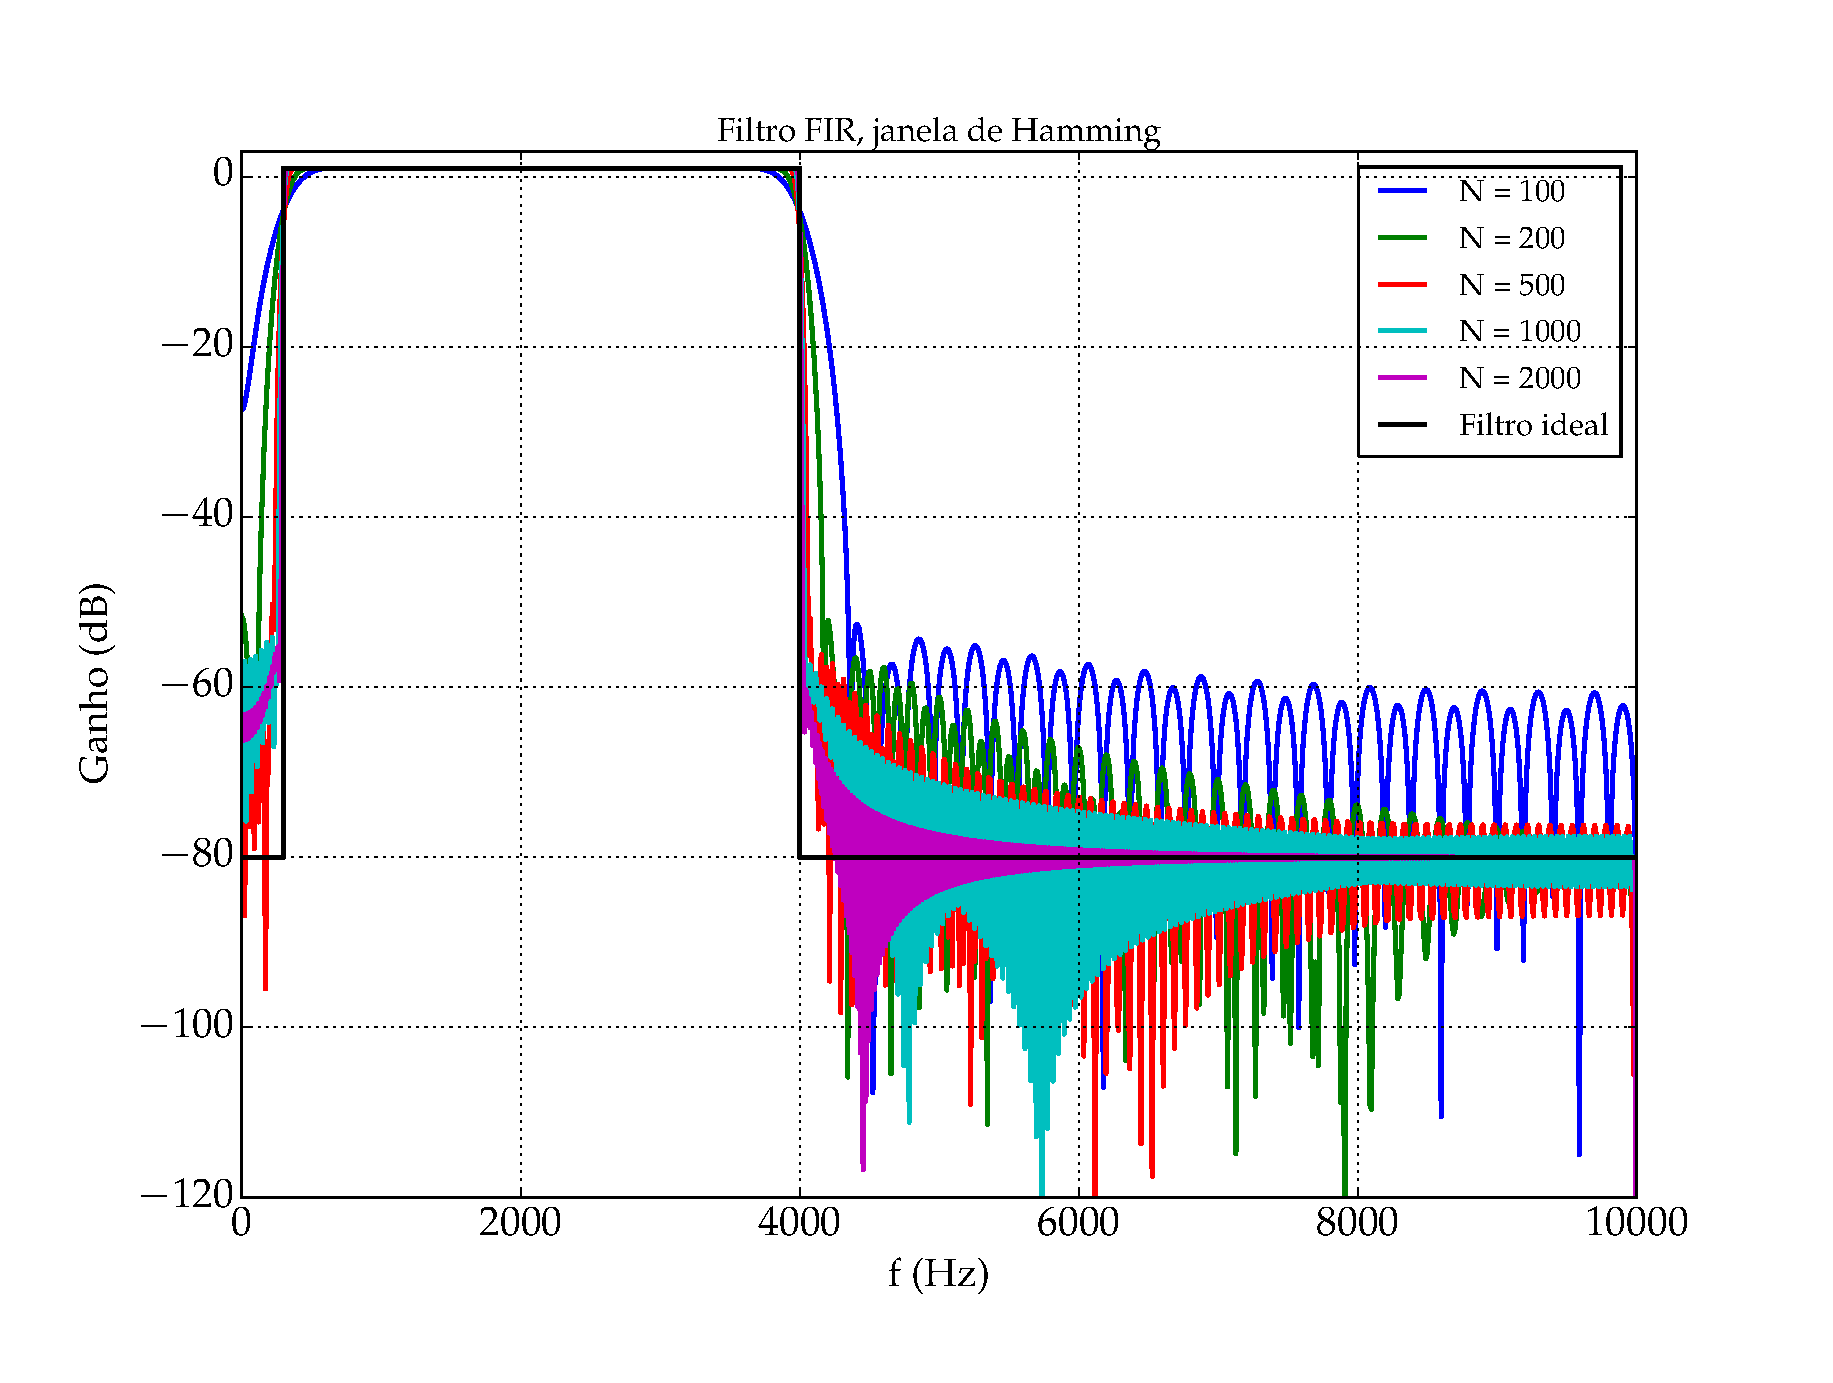
\includegraphics[scale=0.55]{images/plots/bandpass_FIR_hamming_window}
  \caption{Resposta em frequência para filtro band-pass FIR com a função janela de Hamming.}
  \label{fig:bandpass_FIR_hamming}
\end{figure}

\begin{figure}[H]
  \centering
  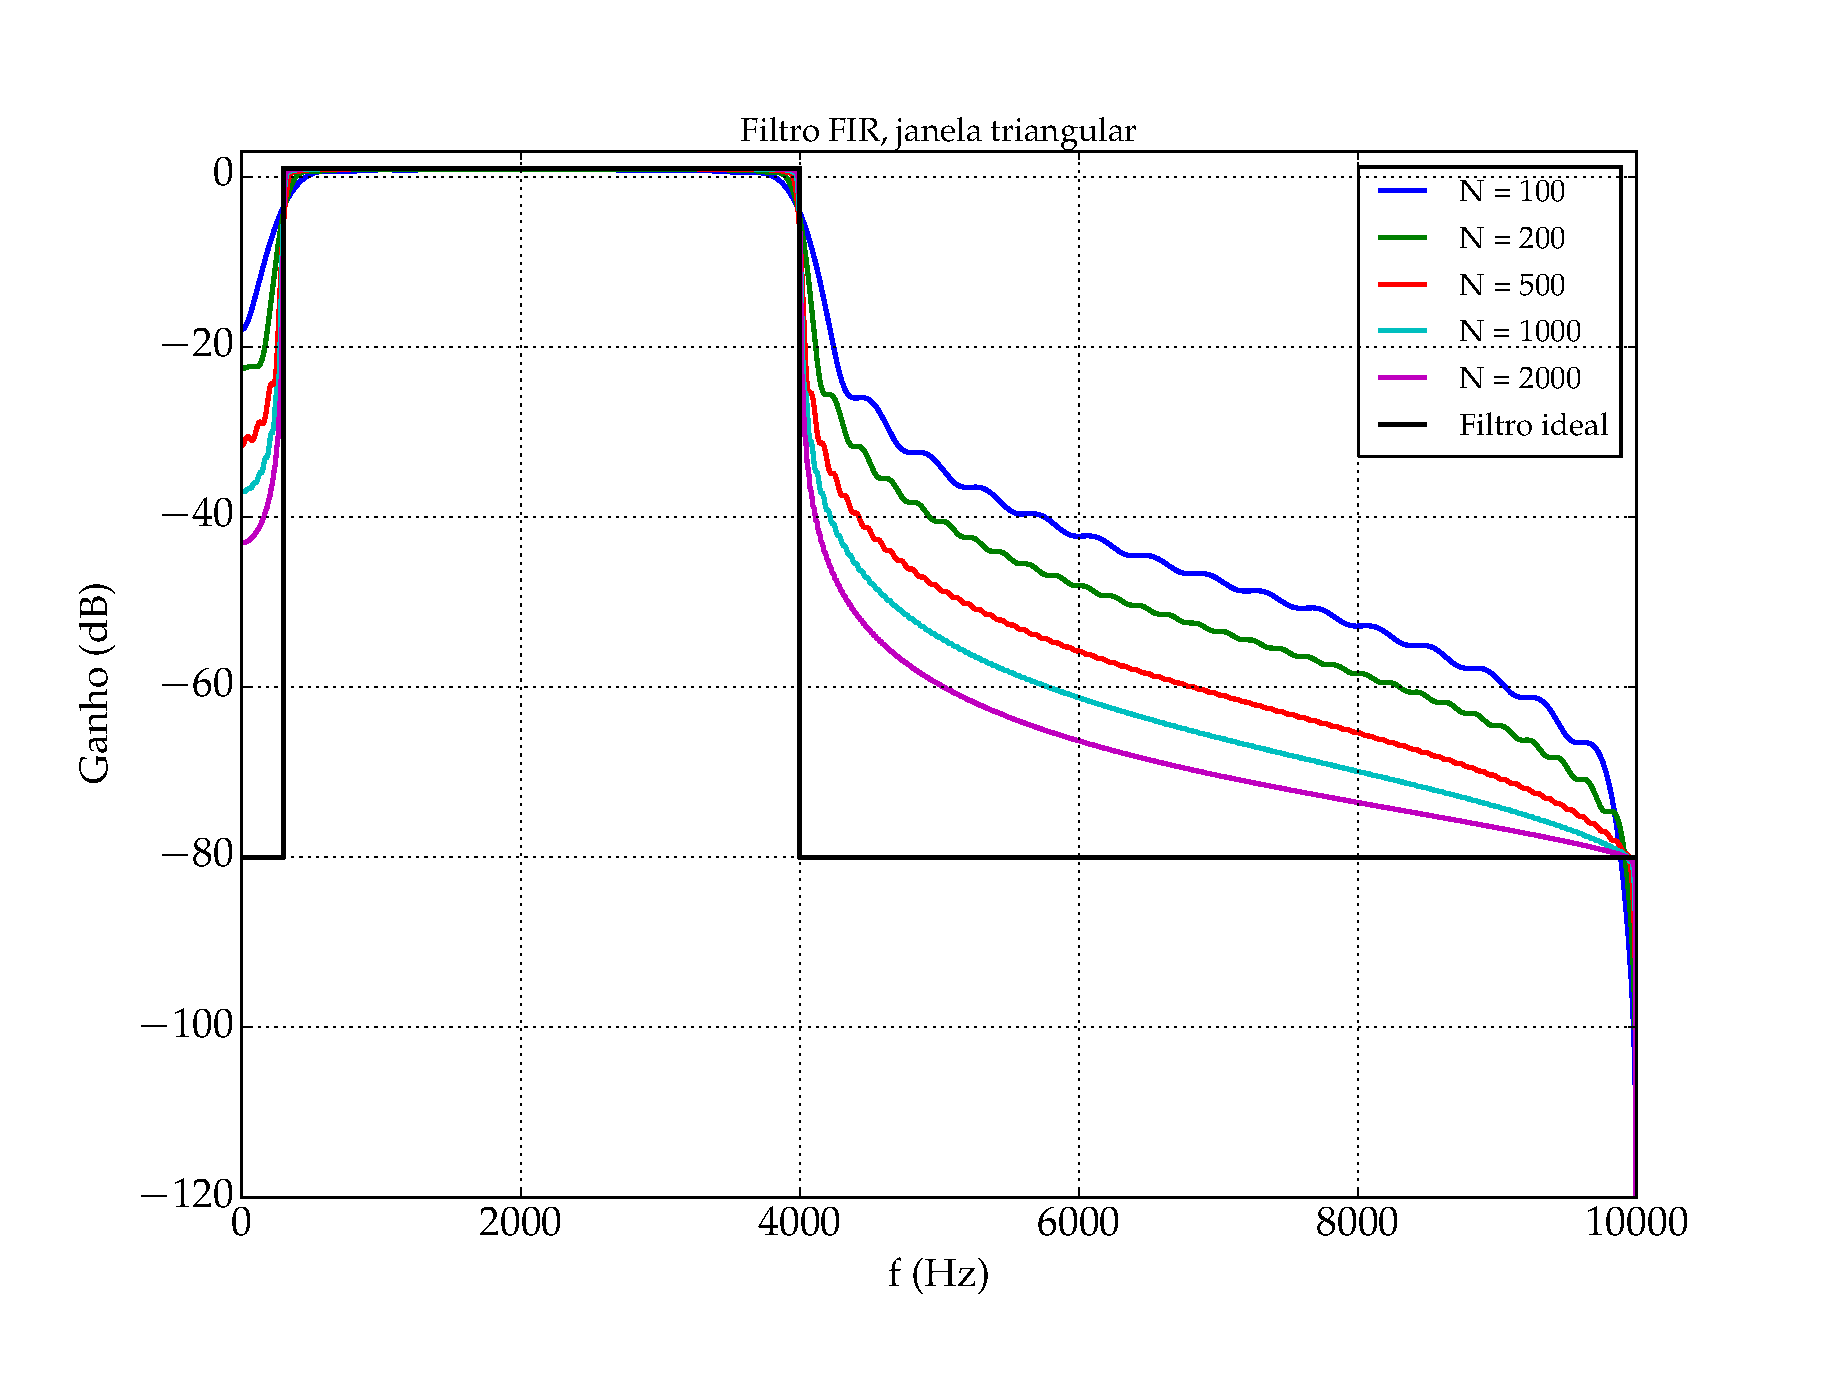
\includegraphics[scale=0.55]{images/plots/bandpass_FIR_triang_window}
  \caption{Resposta em frequência para filtro band-pass FIR com a função janela triangular.}
  \label{fig:bandpass_FIR_triangular}
\end{figure}

É interessante notar que a implementação FIR para esse filtro permite obter uma resposta bem próxima da ideal. Com a função janela de Hamming e a retangular, temos oscilações na banda de parada, ao passo que, empregando-se a janela triangular, estas não acontecem ao custo de uma transição menos ágil.

A partir dos resultados obtidos para os três projetos, os quais confirmam aquilo que foi afirmado na revisão teórica, verifica-se o funcionamento adequado da ferramenta para aquilo que foi proposto no início deste trabalho.

\newpage

\section{Tempo de Processamento}
Como os filtros analógicos e IIR, conforme observado no desenvolvimento deste trabalho, são implementados por meio da aplicação direta de fórmulas, seu tempo de processamento é desprezível e não será abordado. 

Determinam-se os seguintes tempos de processamento para o projeto de filtros FIR, quando executado para um filtro simples em um computador com CPU Intel Core i7 rodando a 2.2 GHz, com 6 GB de RAM e rodando o Linux Ubuntu 15.04 com Python 3.4.3:

% Tive que converter o EPS para PDF, senão o ShareLaTeX dava algum bug que corrompia o arquivo. 
\begin{figure}[H]
  \centering
  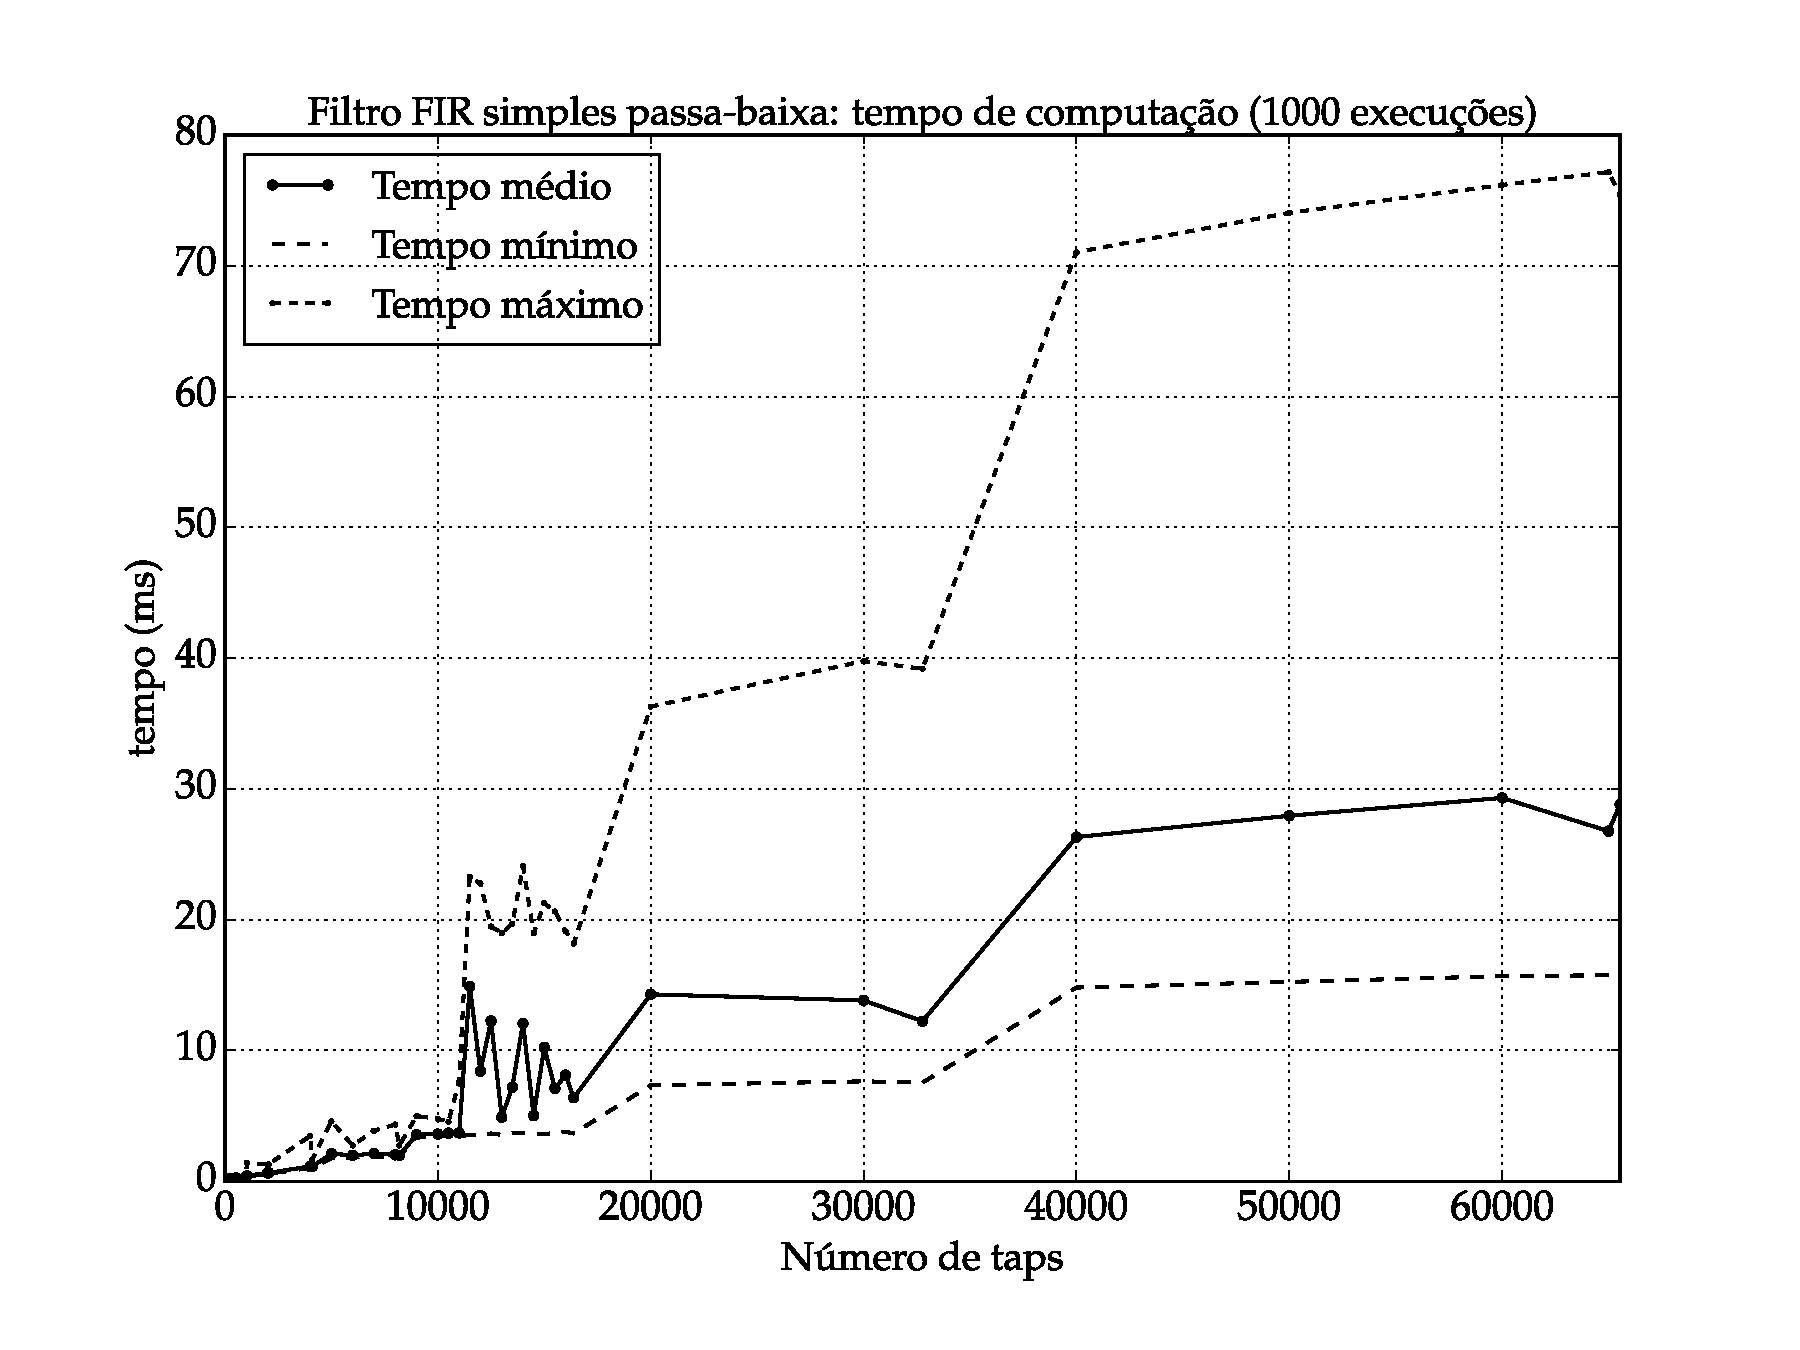
\includegraphics[scale=0.5]{images/plots/fir_benchmark}
 \caption{Tempo de processamento necessário para o projeto de um filtro FIR com N \textit{taps}, pelo método do janelamento. Para cada N o algoritmo foi executado 1000 vezes.}
 \label{fig:fir_benchmark}
\end{figure}

\newpage
Para comparação, um filtro similar foi projetado empregando-se o \textit{MATLAB} versão R2013a no mesmo computador, tendo sido obtido o seguinte resultado:

\begin{figure}[H]
  \centering
  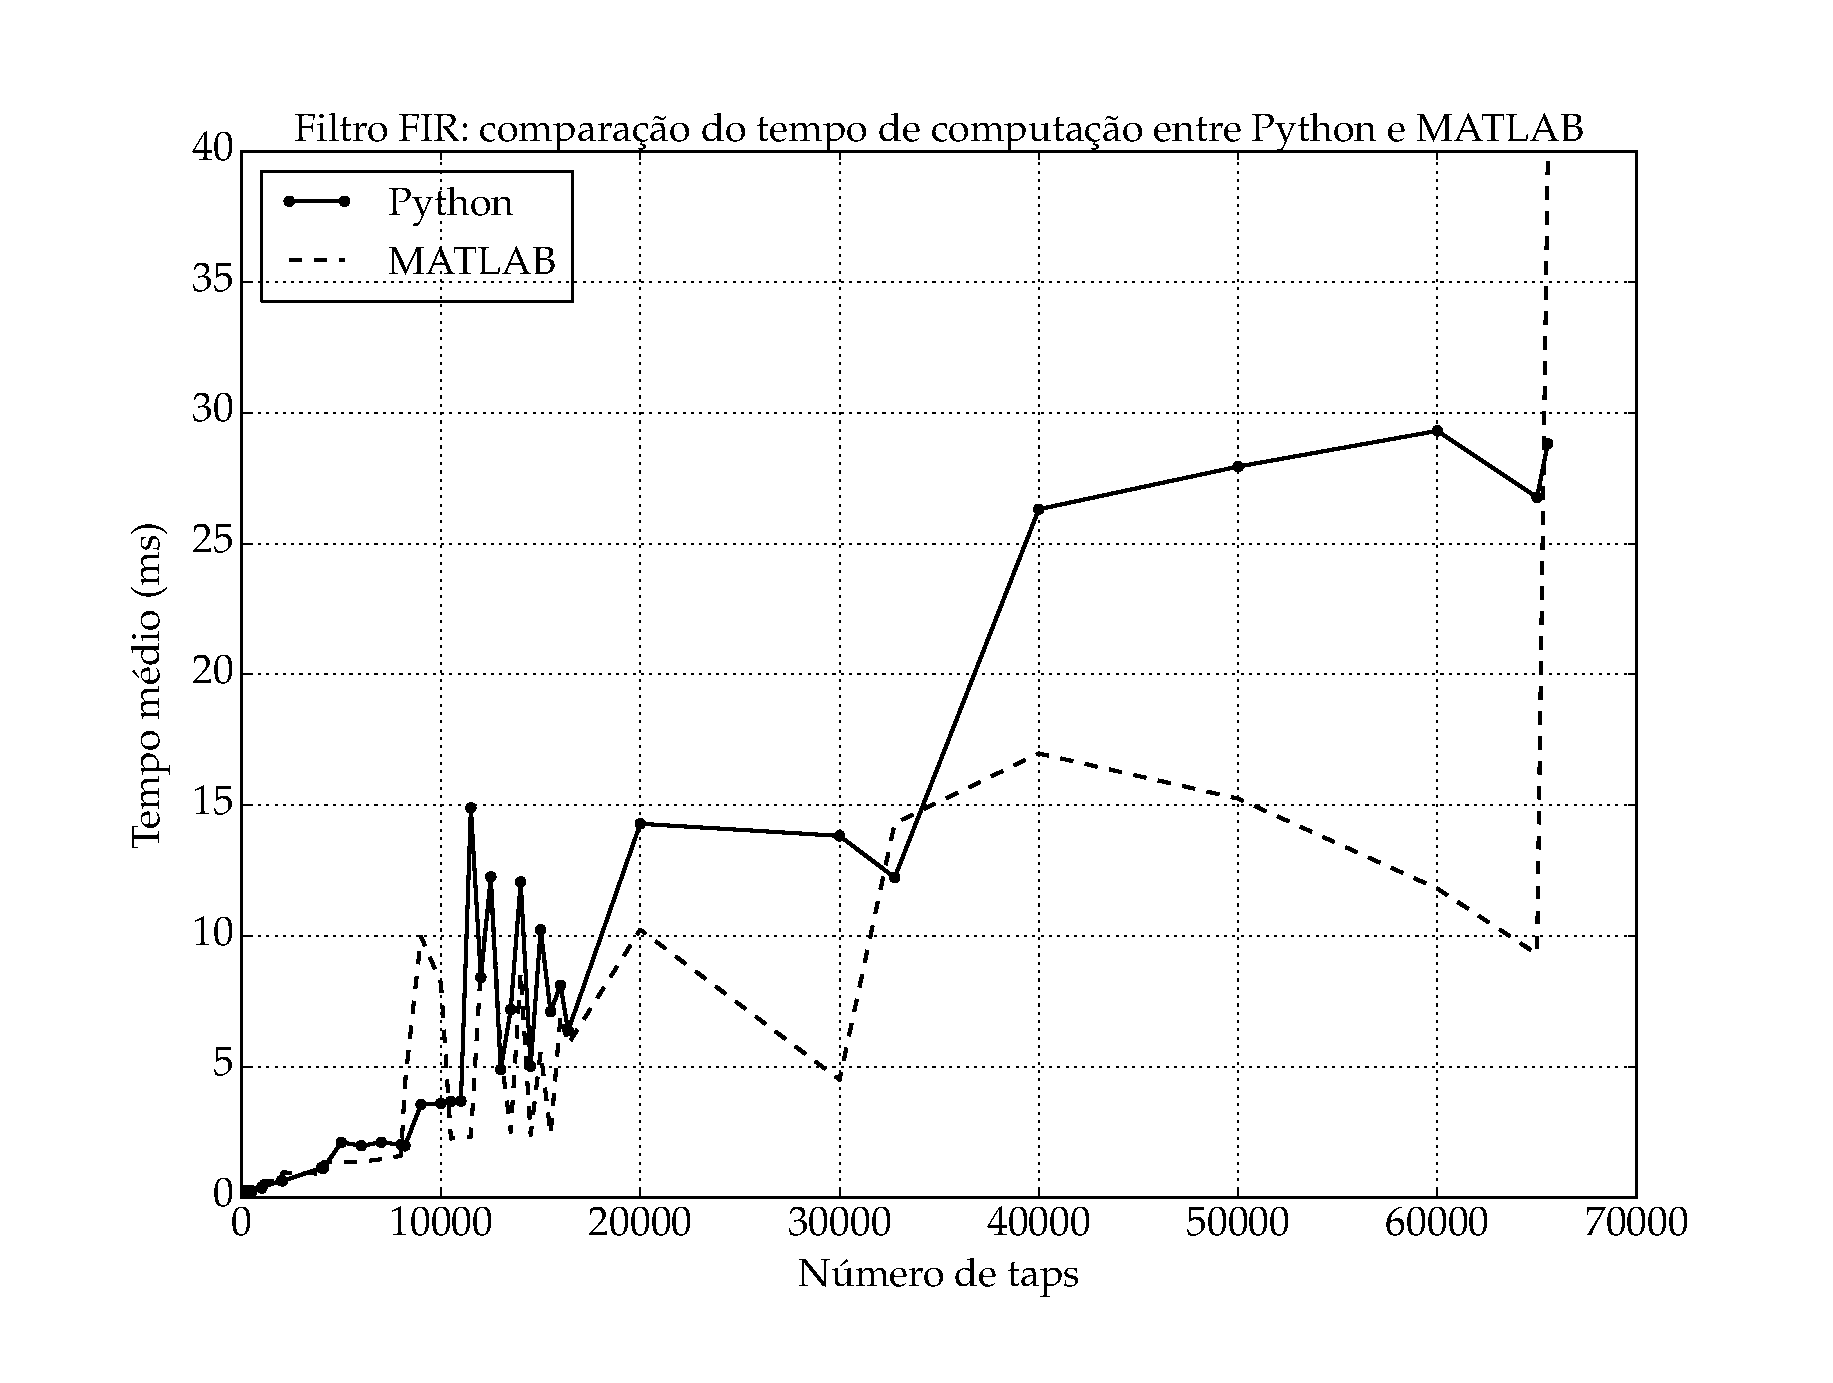
\includegraphics[scale=0.5]{images/plots/fir_comparison}
 \caption{Comparação do tempo tempo de processamento necessário entre Python e MATLAB para o projeto, com as mesmas condições do item \ref{fig:fir_benchmark}.}
 \label{fig:fir_comparison}
\end{figure}


A partir do gráfico \ref{fig:fir_benchmark}, podemos afirmar que o tempo de processamento gasto cresce de forma aproximadamente exponencial com o número de \textit{taps} desejado. Já em \ref{fig:fir_comparison}, verifica-se que o MATLAB apresenta desempenho idêntico ou melhor ao Python; presume-se que esse fenômeno ocorre devido ao fato do MATLAB ter diversas otimizações em suas bibliotecas, porém não é possível confirmar essa hipótese visto que o MATLAB é um \textit{software} de código fechado.

\section{Comparação com Ferramentas já Existentes}
\label{sec:tool_comparison}
Para guiar o desenvolvimento das funcionalidades da ferramenta elaborada no presente trabalho, realizou-se um estudo com algumas das diversas ferramentas já existentes no mercado. 

Para o caso dos filtros analógicos, elas fornecem o circuito projetado; já para os filtros digitais, os coeficientes são fornecidos.  

Também nota-se que o fluxo de trabalho em todas elas é similar: a partir das especificações desejadas, determinam-se funções de transferência ou circuitos que as implementam. 

\subsection{Analog Filter Wizard (Analog Devices)}
Esta ferramenta gratuita, disponível em \cite{analog} é voltada ao projeto de filtros analógicos e implementa os filtros de Bessel, Butterworth e Chebyshev tipo I, com ordens limitadas a 10, permitindo ao usuário decidir entre menos estágios e menor tempo de acomodação.

Uma função interessante dessa ferramenta é permitir algumas otimizações para o circuito (por exemplo, menor consumo de energia ou menor ruído) e realizar a análise das tolerâncias dos componentes: pode-se verificar como o circuito irá se comportar perante a variabilidade dos resistores e capacitores empregados.

\begin{figure}[H] 
\centering 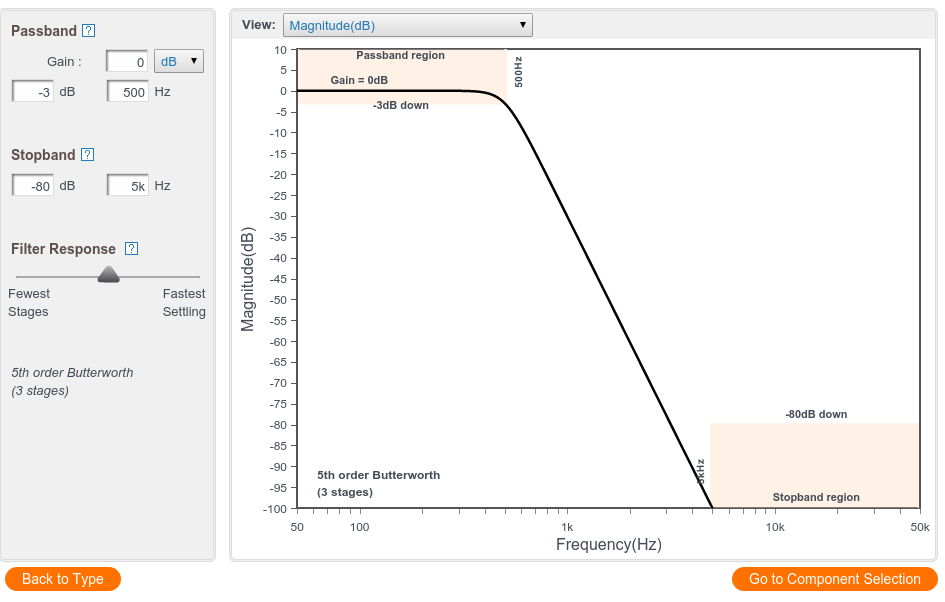
\includegraphics[scale=0.33]{images/screens/afd_in}
\centering 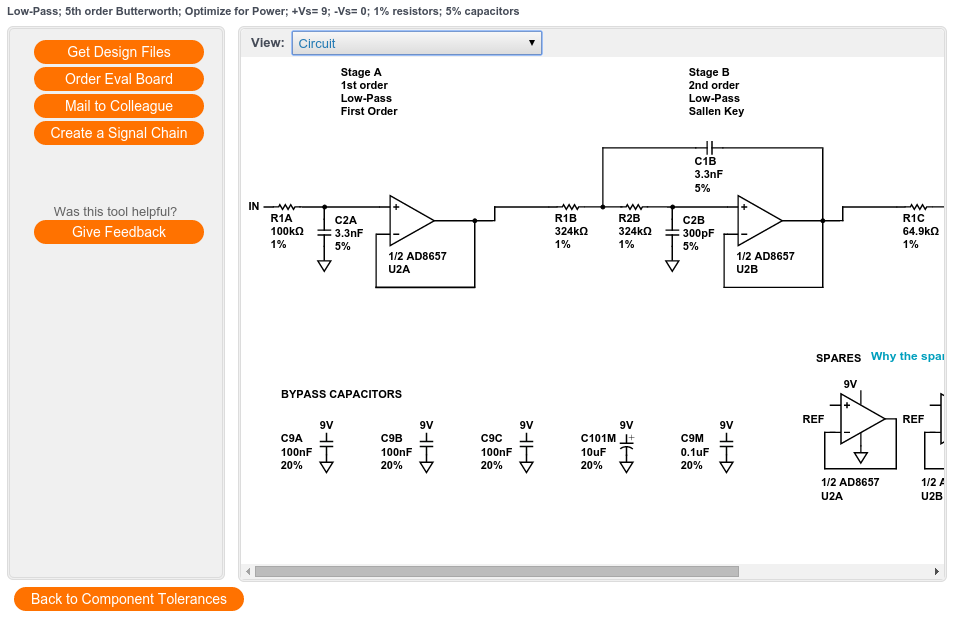
\includegraphics[scale=0.33]{images/screens/afd_out}
\caption{Exemplo da interface do \textit{Analog Filter Wizard}: entrada de dados e resultados.} 
\label{fig:afw_example} 
\end{figure}

\subsection{FilterPro (Texas Instruments)}
Esta ferramenta disponível em \cite{ti_filter} roda no \textit{browser} (é escrita em \textit{Flash}) e permite diversas otimizações no circuito projetado (reduzir o número de componentes ou o custo desses, maximizar a atenuação na banda de parada, minimizar o \textit{ripple} na banda de passagem). 

Assim como o \textit{Analog Filter Wizard}, os circuitos são implementados utilizando-se as topologia \textit{multiple feedback} ou \textit{Sallen-Key.}

\begin{figure}[H] 
\centering 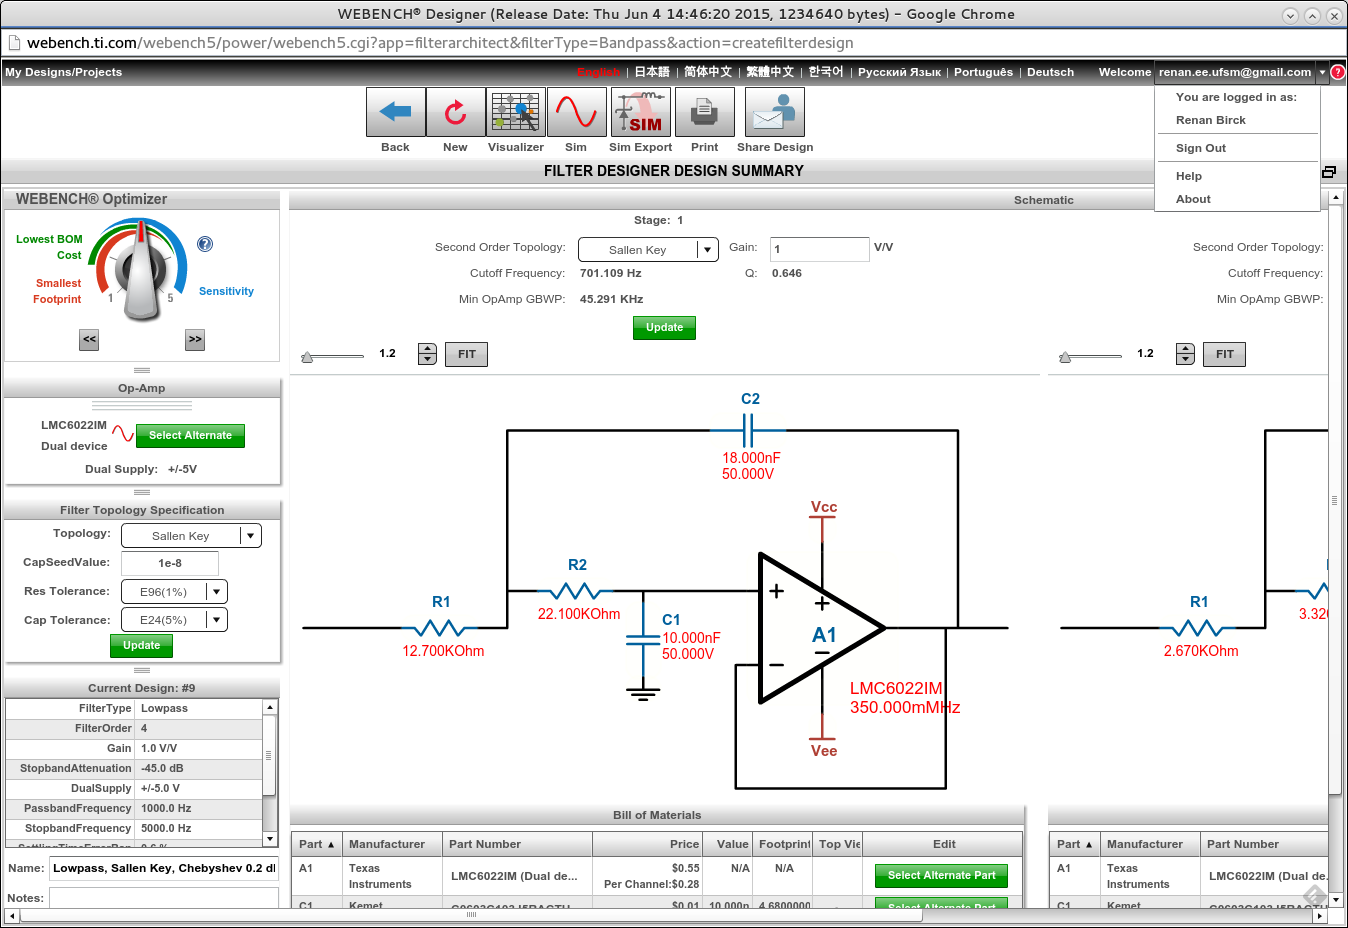
\includegraphics[scale=0.33]{images/screens/fp_example} \caption{Exemplo da interface do \textit{FilterPro}.} 
\label{fig:fp_example} 
\end{figure}

\subsection{DSP System Toolbox (MATLAB)}

Este pacote de ferramentas disponível para o MATLAB é voltado ao projeto de filtros digitais, sendo o mais completo dentre as ferramentas analisadas e cobrindo tanto filtros FIR quanto IIR - para os quais estão implementadas diversos algoritmos de cálculo (método da janela, Parks-McClellan, mínimos quadrados etc...).

Pode ser operado em linha de comando e por meio de interface gráfica, sendo que seu funcionamento e a funcionalidade são similares em ambos; enquanto a interface gráfica permite o projeto interativo, a linha de comando permite o emprego dos filtros projetados em rotinas mais complexas para processamento de sinais.

Uma das suas funcionalidades mais relevantes, considerado que filtros digitais são amplamente empregados em sistemas embarcados, é a sua capacidade de gerar código-fonte em C e em VHDL para uso em CPUs.

\begin{figure}[H] 
\centering 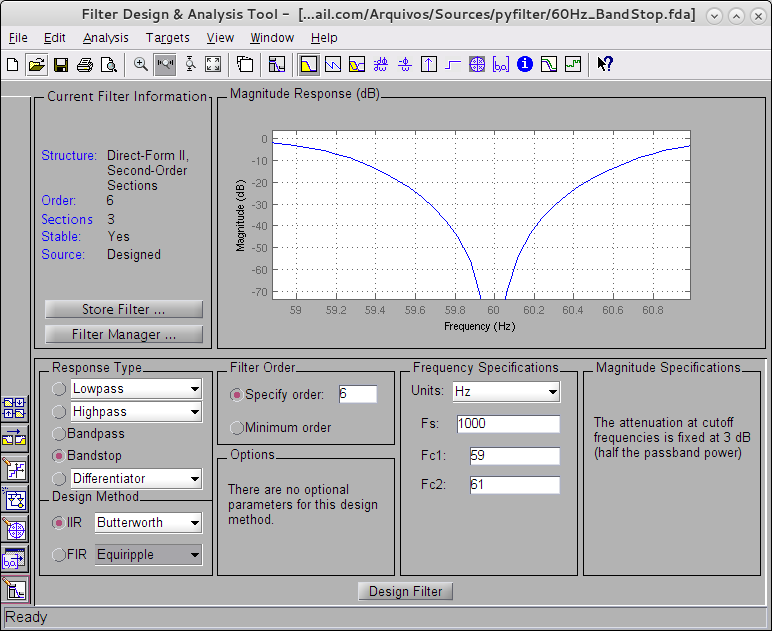
\includegraphics[scale=0.5]{images/screens/fdatool_example} \caption{Exemplo da interface do \textit{Filter Design and Analysis tool}.} 
\label{fig:fda_example} 
\end{figure}

Comparado às ferramentas existentes, a ferramenta apresentada no presente trabalho tem como principal vantagem não ter limitações de ordem do filtro projetado (excetuando-se, conforme descrito no desenvolvimento, o filtro de Bessel que é implementado por meio de tabelas que vão apenas até a 25\textsuperscript{a} ordem).

Outro importante aspecto é que as ferramentas acima descritas são \textit{caixas pretas} de código fechado. Embora, para o usuário, isso muitas vezes não seja um fator limitante ou incômodo, sua funcionalidade está restrita àquela que os desenvolvedores da ferramenta implementaram: há pouca ou nenhuma possibilidade de expansão ou de integração em um algoritmo ou aplicação mais complexa.

A ferramenta desenvolvida aqui, entretanto, tem seu código aberto (\textit{open source}) e também baseada em bibliotecas abertamente disponíveis. Dessa forma, além da vantagem imediata do custo \footnote{Uma licença do MATLAB com as bibliotecas de processamento de sinais e de DSP custa em média US\$ 5 mil}, ela pode ser modificada e expandida pelos seus usuários, que podem adicionar novas funcionalidades e estudar seu código-fonte para entender o funcionamento.

Todavia, não foram implementadas todas funcionalidades existentes nas ferramentas apresentadas: as ferramentas para projeto de filtros analógicos não realizam a síntese de circuitos, já para projeto digital não é gerado código para implementação em uma CPU. No item \ref{sec:improvements} descrevem-se melhorias que podem ser realizadas com o objetivo de dar continuidade a este trabalho e permitir que ele atinja o patamar das ferramentas existentes.